\documentclass[12pt,a4paper]{ctexart}
\usepackage[margin=2.1cm]{geometry}
\usepackage{booktabs}
\usepackage{array}
\usepackage{graphicx}
\usepackage{float}
\usepackage{caption}
\usepackage{subcaption}
\usepackage{hyperref}
\usepackage{siunitx}
\usepackage{xcolor}
\usepackage{amsmath,amssymb}

\title{基于多模态患者级 Attention-MIL 与门控融合的 PTMC 中央区淋巴结转移预测}
\author{PTMC-LNM Study Group}
\date{\today}

\begin{document}
\maketitle

\begin{abstract}
\textbf{目的：}针对 PTMC 中央区淋巴结转移（CentralLNM）术前预测，提出患者级 Attention-MIL、临床主导门控融合与先验约束（$P_{central}\le P_{lnm}$）的统一框架，并与既有基线和消融进行系统对照。\\
\textbf{方法：}在统一患者级 5-fold 协议下，构建 Bag 数据（同一患者多切面），共享实例编码器提取切面特征，经（Mean/Attention）MIL 聚合得到影像患者向量；临床 CSV 由 MLP 编码，经门控融合与影像向量结合，最后由双头输出 LNM 与 CentralLNM；训练时叠加先验约束损失。\\
\textbf{结果：}完整方案（Attention-MIL + Gated + Prior）在 CentralLNM 上达到 \textbf{AUC=0.6963$\pm$0.0115}，且逻辑依从率 \textbf{0.9768$\pm$0.0168}。去除先验后依从率显著下降；门控相对直接拼接更稳。\\
\textbf{结论：}患者级 MIL、门控融合与先验约束能在保证临床一致性的同时提升稳定性，为后续多中心研究提供可复现基线。
\end{abstract}

\tableofcontents
\newpage

\section{引言}
简述 PTMC CentralLNM 预测的重要性、既往方法在外推稳定性上的挑战，并引出本文方法的三个关键要素：患者级 MIL、临床主导门控融合、先验约束损失。

\section{相关工作}
多实例学习（MIL）在医学影像中的应用；多模态融合策略（拼接、门控、注意力）；基于临床先验的结构化损失或约束。

\section{方法}
\subsection{数据与患者级 Bag 构建}
将同一患者的所有对齐切面聚合为一个 Bag；标签为患者级 CentralLNM、LNM。
\subsection{实例编码与 MIL 聚合}
共享 CNN 提取切面向量 $h_i$；Attention-MIL 计算 $a_i$ 并加权求和 $H_{img}=\sum a_i h_i$；Mean-MIL 作为对照。
\subsection{临床特征编码与门控融合}
临床向量经 MLP 得到 $H_{clin}$；门控 $G=\sigma(W H_{clin}+b)$ 控制影像信息注入：$H_{final}=H_{clin}+G\odot H_{img}$；直接拼接作为对照。
\subsection{先验约束损失}
惩罚违反 $P_{central}\le P_{lnm}$ 的样本：$L_{pen}=\mathrm{mean}\,\mathrm{ReLU}(P_{central}-P_{lnm})$，总损失叠加 $\alpha L_{pen}$。


\subsection{Attention-MIL 机制}
在患者级 MIL 框架中，一个患者被视为一个“包”（bag），包含 $N$ 个实例（切面）及其多模态输入。首先以共享 CNN 对每个实例提取嵌入 $h_i\in\mathbb{R}^D$；随后用门控注意力计算实例权重：
\begin{equation}
 a_i = \mathrm{softmax}_i\!\left(\, w^\top\!\left[\tanh(Vh_i) \odot \sigma(Uh_i)\right] \right), \quad
 H_{img}=\sum_{i=1}^{N} a_i h_i.
\end{equation}
其中 $H_{img}$ 为影像患者向量。对照实验中使用 Mean-MIL：$H_{img}=\frac{1}{N}\sum_i h_i$。

\subsection{临床主导的门控融合}
临床向量经 MLP 得到 $H_{clin}$，随后以临床为先导生成门控并控制影像信息注入：
\begin{equation}
 G = \sigma(W_{gate}H_{clin}+b), \quad H_{final}=H_{clin}+G\odot H_{img}.
\end{equation}
该设计用于在不牺牲临床稳定性的前提下，吸收影像信息。对照采用 $[H_{clin};H_{img}]$ 直接拼接的 MLP 融合。

\subsection{先验约束与损失}
为符合“中央区转移概率不应高于整体转移”的临床逻辑，训练时对违反样本施加软惩罚：
\begin{equation}
 L_{pen}=\mathrm{mean}\,\max\!\left(0,\, P_{central}-P_{lnm}\right), \qquad
 L=L_{cls}+\alpha L_{pen}.
\end{equation}
实验发现 $\alpha>0$ 时不仅提升了逻辑依从率，也提升了整体稳定性。

\subsection{ROI影像组学分支与三种融合策略}
为增强三源融合中的影像侧可解释特征，本文引入患者级 ROI Radiomics 分支。具体流程为：
\begin{enumerate}
  \item 基于病灶掩膜做切片级 PyRadiomics 提取；
  \item 在训练集内进行 LASSO 选择，得到患者级组学向量 $V_{rad}$（避免信息泄漏）；
  \item 将组学分支与深度分支进行融合后，再进入临床主导门控模块。
\end{enumerate}

在统一训练协议下比较三种 V2 融合方式：
\paragraph{(1) V2-legacy（原始拼接）}
\begin{equation}
H_{img}^{mix}=\mathrm{MLP}([H_{deep};H_{rad}]), \quad
H_{final}=H_{clin}+G\odot H_{img}^{mix}.
\end{equation}

\paragraph{(2) V2-align\_proj（特征空间对齐投影）}
将深度特征与组学特征投影到同一隐空间（本文设为 128 维）：
\begin{equation}
Z_{deep}=\mathrm{MLP}_{deep}(H_{deep}),\quad
Z_{rad}=\mathrm{MLP}_{rad}(V_{rad}).
\end{equation}
随后做对齐融合（本文使用 concat+MLP）并映射回影像语义空间：
\begin{equation}
Z_{mix}=\mathrm{MLP}_{fuse}([Z_{deep};Z_{rad}]),\quad
H_{img}^{mix}=\mathrm{MLP}_{back}(Z_{mix}).
\end{equation}
最终仍采用临床门控：
\begin{equation}
H_{final}=H_{clin}+G\odot H_{img}^{mix}.
\end{equation}

\paragraph{(3) V2-FiLM（特征调制）}
将组学向量作为调制器，生成深度通道的缩放与偏移参数：
\begin{equation}
\gamma = 1 + s\cdot\tanh(\mathrm{Linear}_{\gamma}(H_{rad})),\quad
\beta = \mathrm{Linear}_{\beta}(H_{rad}),
\end{equation}
\begin{equation}
H_{img}^{mod}=\gamma\odot H_{deep}+\beta,\quad
H_{final}=H_{clin}+G\odot H_{img}^{mod}.
\end{equation}
其中 $s$ 为缩放系数（本文设为 0.1），用于抑制训练早期的过激调制。

\subsection{原始临床回归基线}
除使用预处理临床向量的深度模型外，本文额外构建了更符合医学论文语境的“原始临床回归基线”。具体做法为：直接读取原始临床 Excel，以 `Image` 列与网络训练使用的患者级 5-fold 划分文件对齐，再通过 `HISID` 聚合到患者级，从而保证与深度模型共享完全一致的 train/val/test split。

术前临床候选变量取自 Excel 的 `D\sim Z` 列；标签由淋巴结阳性结节计数列构造：
\begin{itemize}
  \item `LNM`：阳性 LN 总数 $>0$；
  \item `CentralLNM`：中央组 LN 阳性数 $>0$；
  \item `LateralLNM`：侧方 LN 阳性数 $>0$。
\end{itemize}

建模时采用经典临床统计流程：训练集内完成缺失值填补与类别编码，先进行单因素 Logistic 回归筛选，再进入多因素 Logistic 回归，并在 test 集报告 AUC、ACC、F1、Sensitivity、Specificity。该设计的目的不是替代深度模型，而是提供一个基于原始术前变量、且与深度模型在同一患者级 split 上公平对齐的临床参照。
\begin{figure}[H]
  \centering
  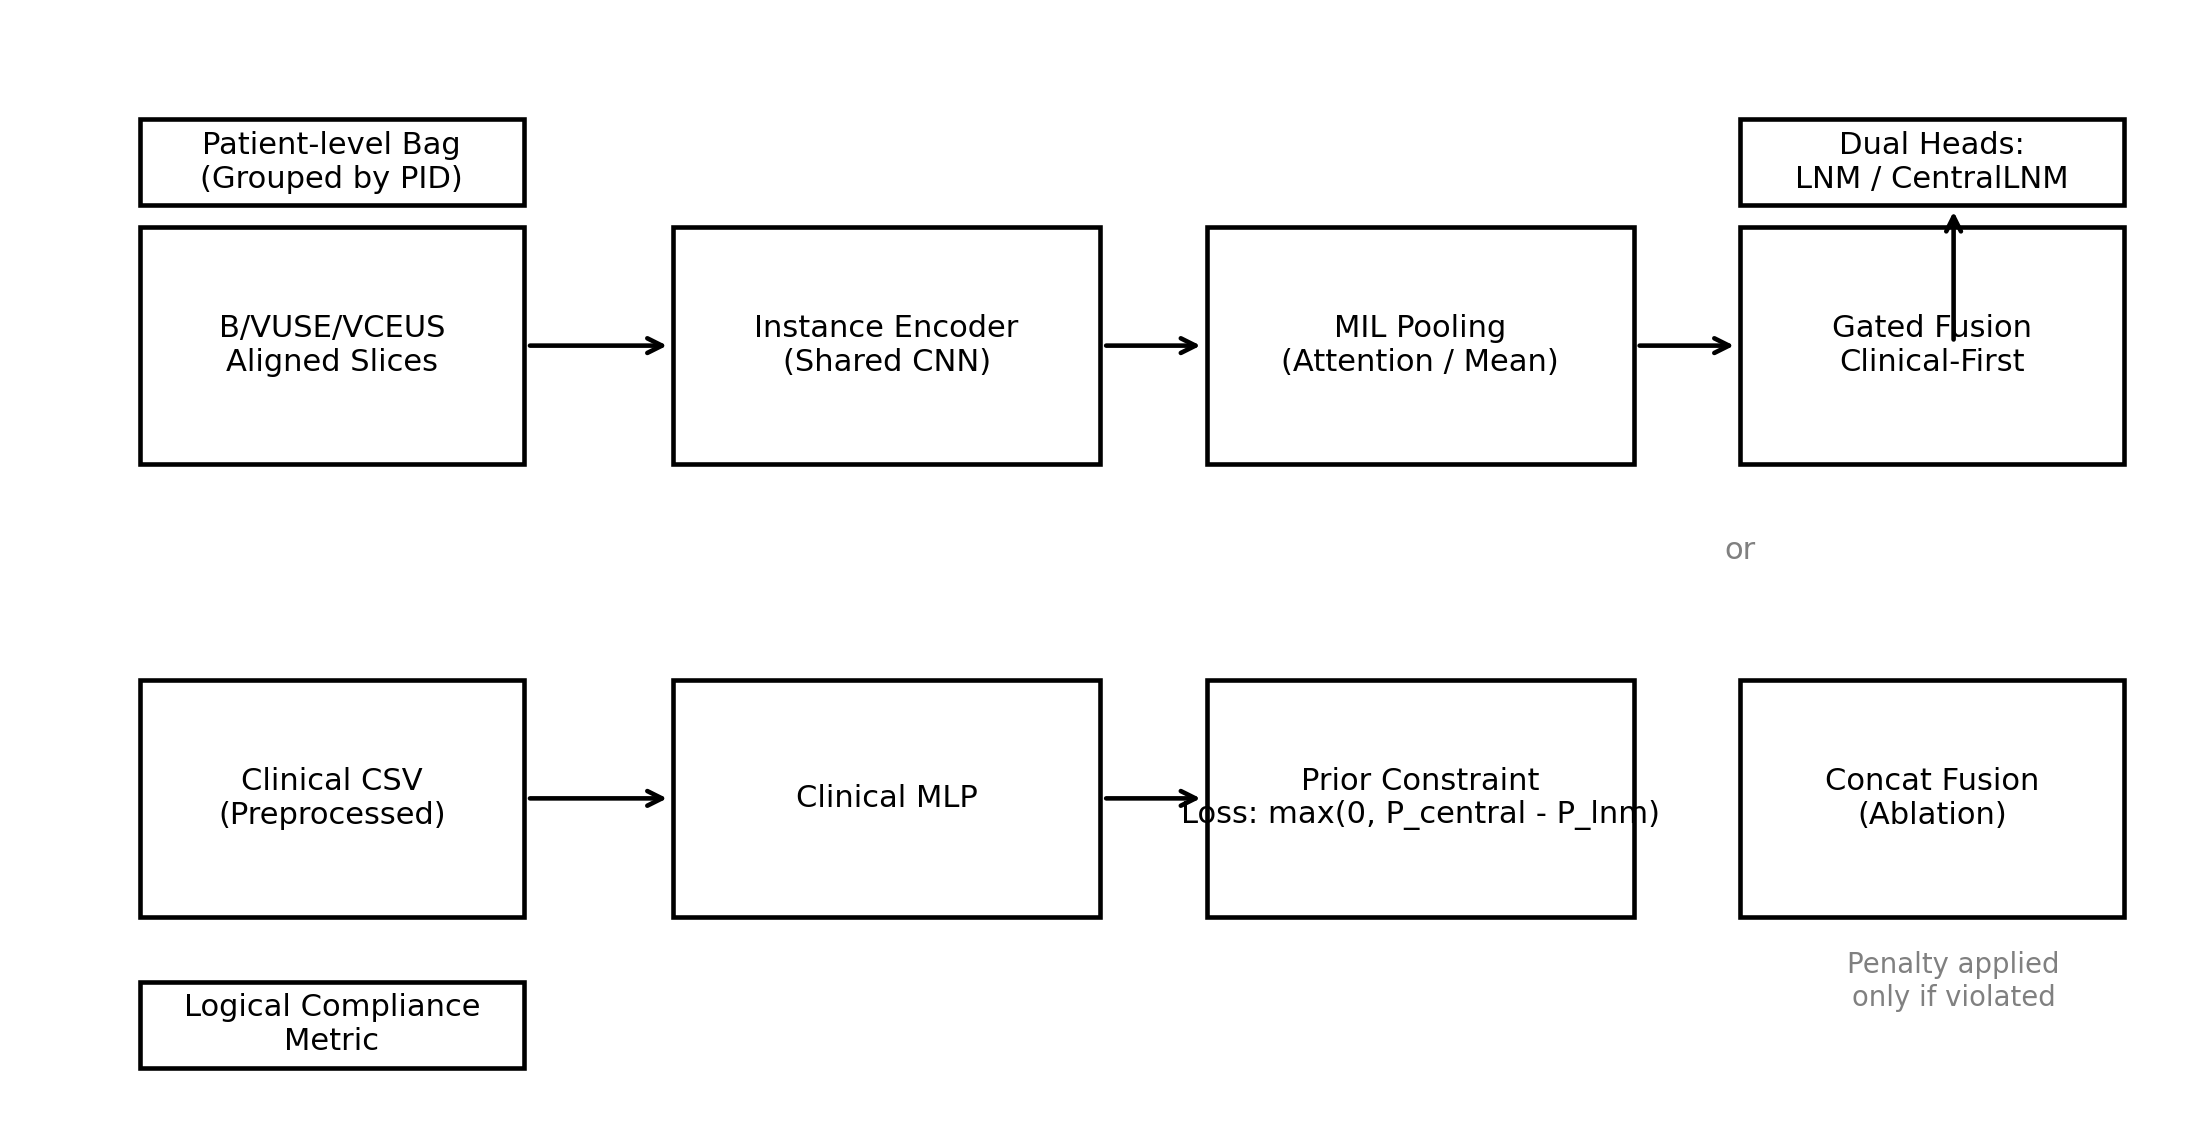
\includegraphics[width=0.95\textwidth]{figures/mil_gated_prior_arch.png}
  \caption{方法总体架构：共享实例编码 +（Mean/Attention）MIL 聚合 + 临床主导门控融合 + 先验约束 + 双任务头。}
\end{figure}

\subsection{方法变量表（主要超参与训练设定）}
\begin{table}[H]
\centering
\caption{主要超参数与训练设置}
\begin{tabular}{p{0.34\textwidth}p{0.58\textwidth}}
\toprule
项目 & 设置 \\
\midrule
数据划分 & 患者级 5-fold（\texttt{groups\_cv5\_central}） \\
输入模态 & B + VUSE + VCEUS（多模态通道拼接） \\
图像尺寸 / 每患者最大实例数 & 224$\times$224 / 12 \\
主干网络 & ResNet18（ImageNet 预训练，前3个 epoch 冻结） \\
MIL 聚合 & Attention-MIL（对照：Mean-MIL） \\
融合方式 & Clinical-first Gated Fusion（对照：Concat Fusion） \\
任务头 & 双任务：LNM 与 CentralLNM \\
损失函数 & BCE(LNM)+BCE(Central)+$\alpha\cdot\max(0,P_{central}-P_{lnm})$ \\
先验权重 $\alpha$ & Ours=1.0（消融：$\alpha=0$） \\
优化器 / 学习率 & AdamW，$lr=1e{-4}$，$lr_{backbone}=1e{-5}$ \\
训练轮数 / 早停 & 最多60 epoch，patience=15 \\
评估指标 & AUC、ACC、F1、Sensitivity、Specificity、Logical Compliance \\
\bottomrule
\end{tabular}
\end{table}

\section{实验设置}
\subsection{数据与划分}
沿用原项目患者级 5-fold 划分与评估；CentralLNM 为主终点。
\subsection{评价指标}
报告 AUC（均值$\pm$std），并给出 ACC、F1、Sensitivity、Specificity，及逻辑依从率。
\subsection{对照与消融}
Baseline A（clinical-only）、Baseline B（slice-mean-concat）、Ablation 1（mean-mil-gated）、Ablation 2（attention-mil-concat）、Ablation 3（full $\alpha=0$）、Ours（full $\alpha=1$）。

\section{结果}
\subsection{总体对照（6组消融）}
\begin{figure}[H]
  \centering
  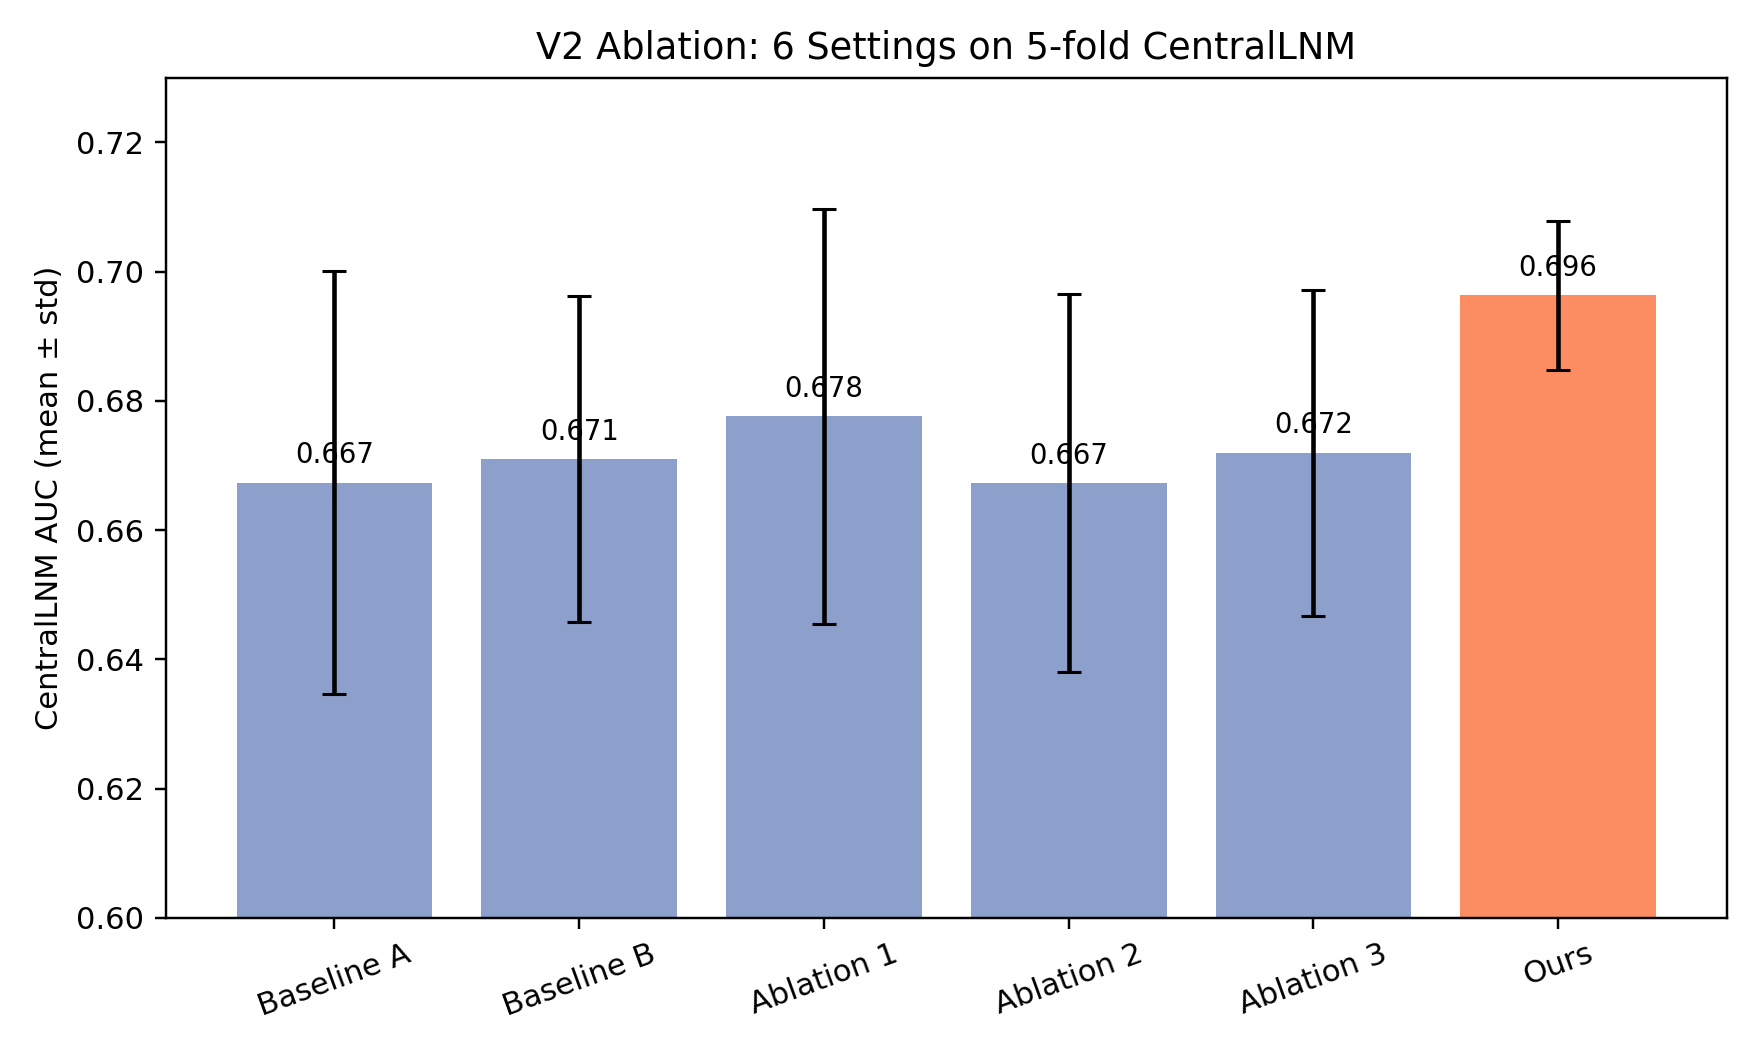
\includegraphics[width=0.92\textwidth]{figures/auc_bar_v2_ablation6.png}
  \caption{6组消融：CentralLNM AUC（5-fold，mean$\pm$std）。}
\end{figure}
\paragraph{图表分析}完整模型（Ours）在均值AUC上最高且标准差最小，说明性能提升与稳定性改进同时成立。
\paragraph{图表分析}相较各消融，Attention-MIL、门控融合与先验约束的组合呈现协同增益，而非单一模块驱动。
\begin{figure}[H]
  \centering
  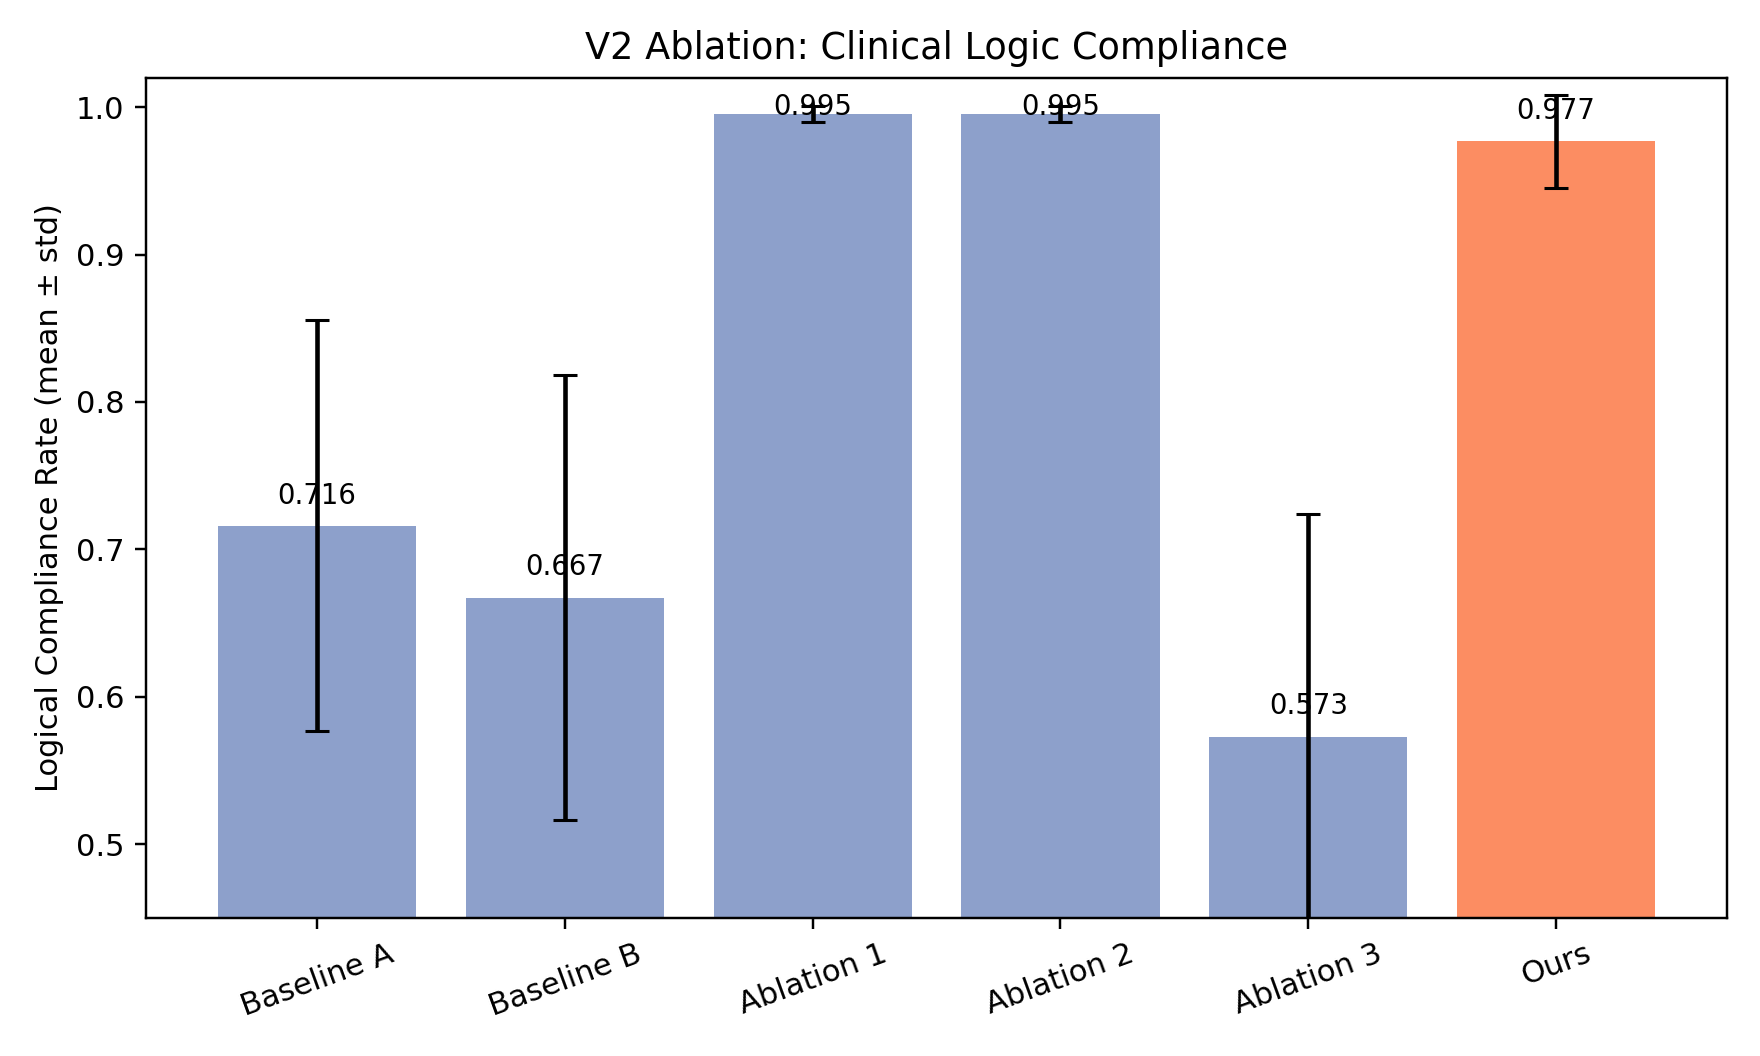
\includegraphics[width=0.92\textwidth]{figures/compliance_bar_v2_ablation6.png}
  \caption{6组消融：临床逻辑依从率（$P_{central}\le P_{lnm}$）。}
\end{figure}
\paragraph{图表分析}加入先验约束后依从率显著提升，去除先验（Ablation 3）后依从率明显下滑。
\paragraph{图表分析}Ours 在高依从率下仍维持最佳AUC，说明临床一致性约束并未牺牲判别性能。
\subsection{总体全指标对照表}
\begin{table}
\centering
\caption{六组消融的全指标对照（5-fold test）}
\label{tab:ablation_full_metrics}
\small
\begin{tabular}{lcccccc}
\toprule
                                  设置 &             AUC &      ACC &       F1 &  Sensitivity &  Specificity &      Compliance \\
\midrule
                      Base-A (Clin) & 0.667$\pm$0.033 & 0.610274 & 0.626488 &     0.625069 &     0.592692 & 0.716$\pm$0.140 \\
               Base-B (SliceMean+Cat) & 0.671$\pm$0.025 & 0.596343 & 0.662652 &     0.735430 &     0.432051 & 0.667$\pm$0.151 \\
                     Abl-1 (MeanMIL+G) & 0.678$\pm$0.032 & 0.626499 & 0.632109 &     0.607493 &     0.650385 & 0.995$\pm$0.006 \\
                     Abl-2 (AttMIL+Cat) & 0.667$\pm$0.029 & 0.614761 & 0.656433 &     0.684181 &     0.532692 & 0.995$\pm$0.006 \\
                      Abl-3 (NoPrior) & 0.672$\pm$0.025 & 0.587122 & 0.638122 &     0.693247 &     0.462308 & 0.573$\pm$0.151 \\
                        Ours (AttMIL+G+P) & 0.696$\pm$0.012 & 0.624359 & 0.674504 &     0.717761 &     0.513718 & 0.977$\pm$0.032 \\
\bottomrule
\end{tabular}
\end{table}

\paragraph{关键观察}Ours 在 AUC 与逻辑依从率上同时占优；Ablation 1 高于 Ablation 2，提示“门控融合”较“直接拼接”更稳健；去除先验（Ablation 3）后依从率明显劣化，验证了先验约束对临床一致性的必要性。
\paragraph{临床解读}本任务的模型选择不应仅看 AUC，还需同时关注灵敏度下限与依从率。对于术前筛查场景，较高灵敏度通常优先于极致特异度，以降低假阴性带来的漏诊风险。


\subsection{Ours：5-fold ROC 与校准}
\begin{figure}[H]
  \centering
  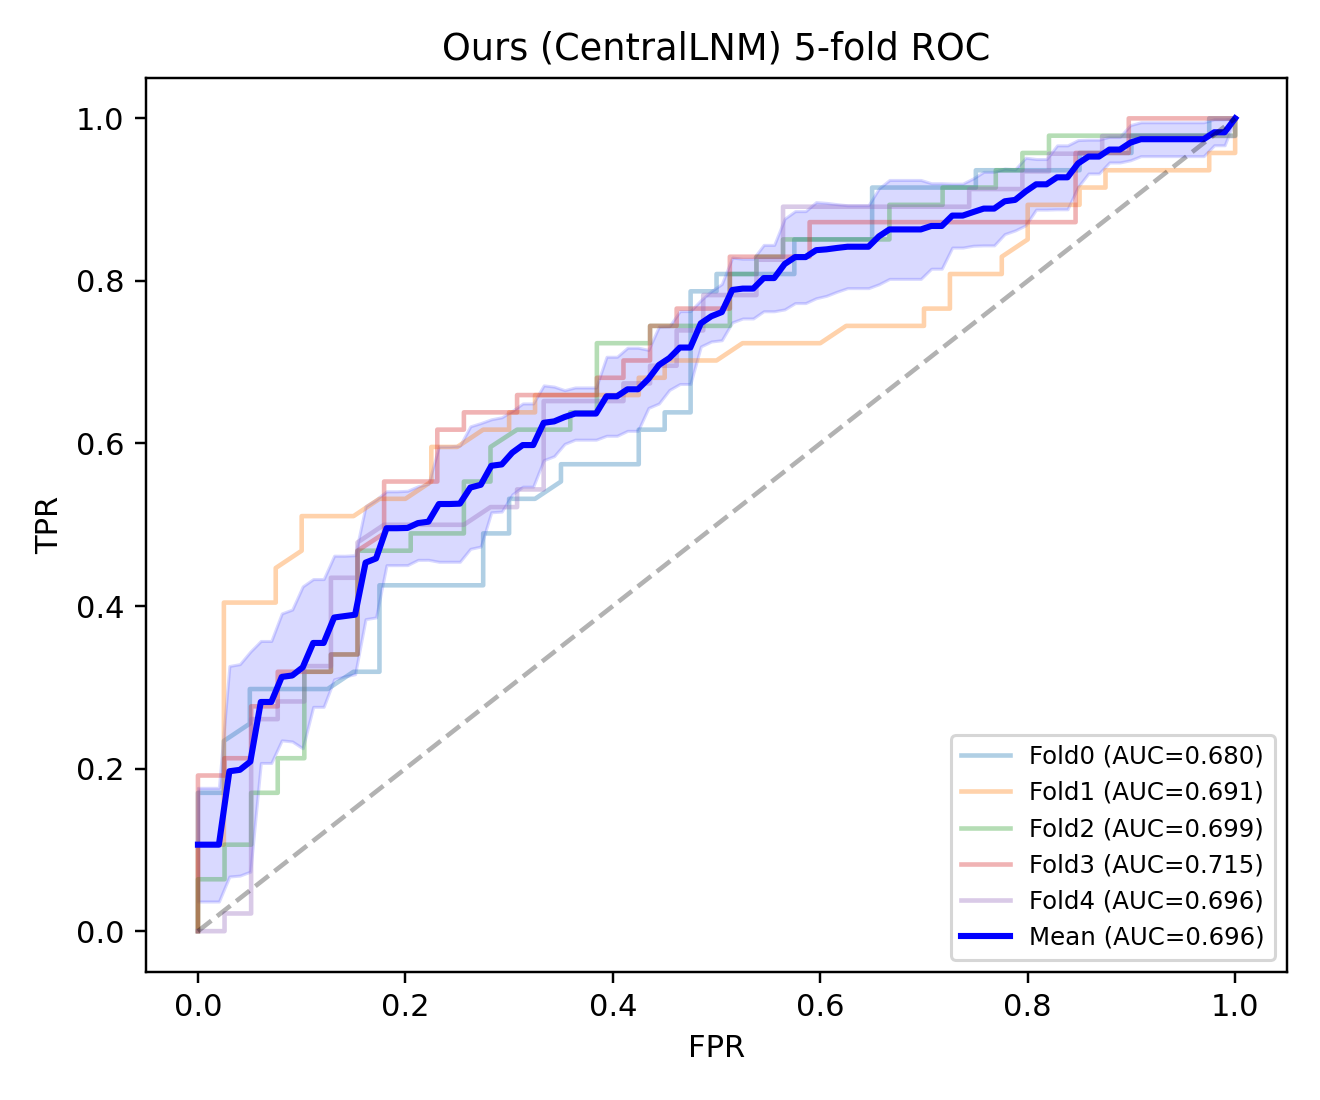
\includegraphics[width=0.78\textwidth]{figures/roc_overlay_ours_full.png}
  \caption{Ours（CentralLNM）患者级 5-fold ROC 叠加与均值曲线。}
\end{figure}
\paragraph{图表分析}5折 ROC 曲线整体围绕均值曲线分布，提示跨折波动可控、泛化较稳定。
\paragraph{图表分析}在中高召回区间仍保持较好特异性，支持作为临床风险分层工具的可行性。
\begin{figure}[H]
  \centering
  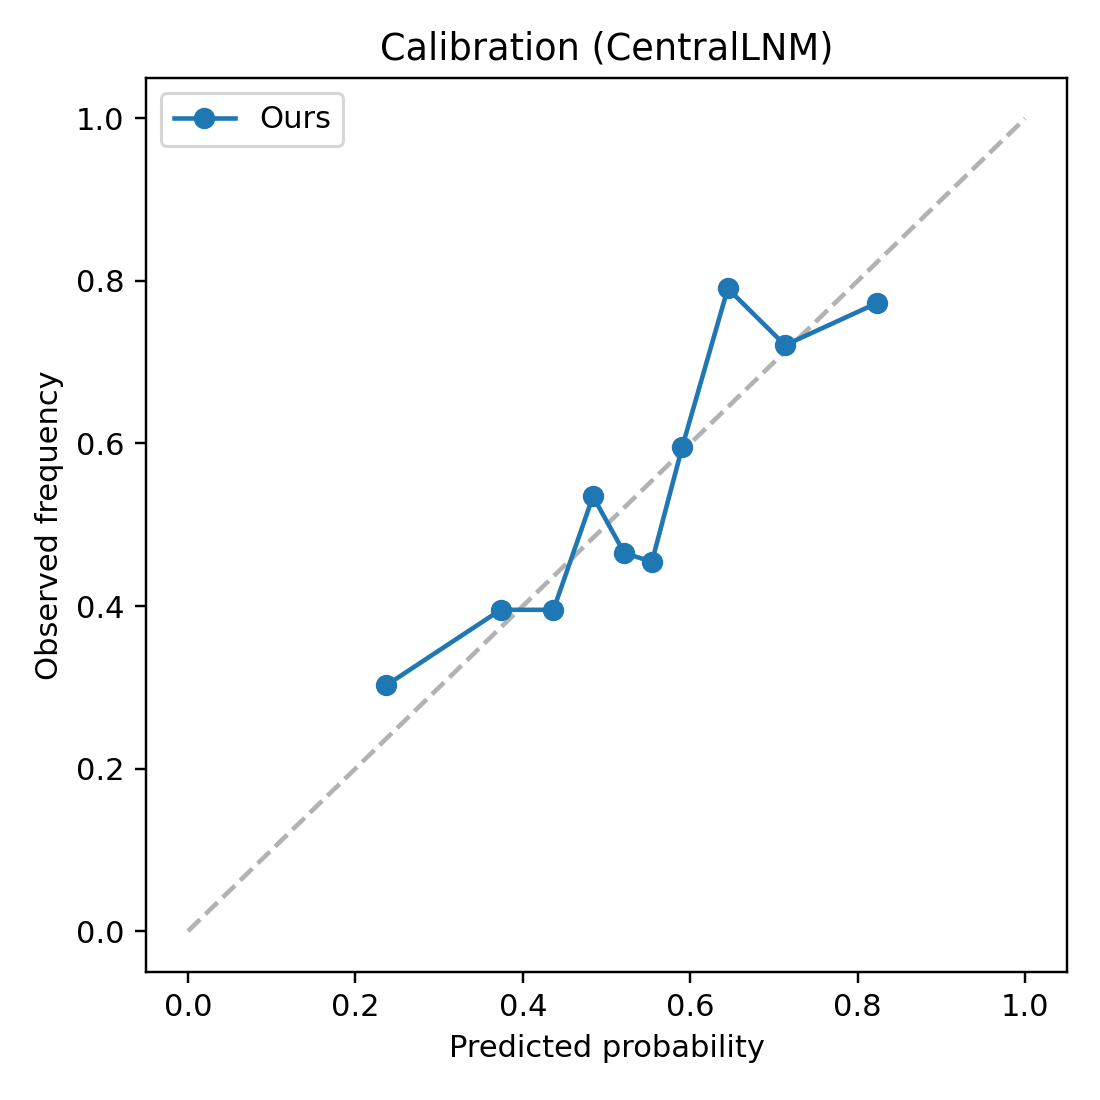
\includegraphics[width=0.60\textwidth]{figures/calibration_ours_full.png}
  \caption{Ours 的可靠性曲线（分位数分箱）。}
\end{figure}
\paragraph{图表分析}可靠性曲线总体贴近对角线，说明预测概率与观测事件率匹配度较好。
\paragraph{图表分析}高风险端仍存在轻微偏移，后续可考虑温度缩放或分层校准进一步优化。

\subsection{不同骨干架构公平对比（8种）}
在保持同一训练协议（同数据划分、同损失项、同优化策略、同训练轮数上限，且统一 \texttt{pretrained=True}）下，对 ResNet、EfficientNet、ConvNeXt、ViT、Swin 与 MobileViT 共 8 种骨干进行对比，结果如下。

\begin{table}[H]
\centering
\caption{8种骨干网络在统一训练协议（pretrained=True）下的患者级5-fold汇总对比（mean$\pm$std）。}
\small
\begin{tabular}{lcccccc}
\toprule
Backbone & Central AUC & ACC & F1 & Sen & Spe & Compliance \\
\midrule
ViT-B/16 & \textbf{$0.7104\pm0.0253$} & 0.6289 & 0.6686 & 0.6969 & 0.5490 & $0.9512\pm0.0626$ \\
MobileViT-S & $0.6995\pm0.0463$ & 0.6244 & 0.6817 & 0.7521 & 0.4740 & $0.9746\pm0.0268$ \\
ResNet18 & $0.6963\pm0.0115$ & 0.6244 & 0.6745 & 0.7178 & 0.5137 & $0.9768\pm0.0317$ \\
Swin-T & $0.6939\pm0.0267$ & 0.6473 & 0.6620 & 0.6635 & 0.6296 & \textbf{$0.9977\pm0.0047$} \\
EffNet-B2 & $0.6861\pm0.0268$ & 0.6170 & 0.6613 & 0.7148 & 0.5022 & $0.9744\pm0.0173$ \\
EffNet-B0 & $0.6732\pm0.0236$ & 0.6173 & 0.6592 & 0.7014 & 0.5178 & $0.9700\pm0.0382$ \\
ConvNeXt-T & $0.6645\pm0.0267$ & 0.6379 & 0.6762 & 0.7179 & 0.5432 & $0.9883\pm0.0148$ \\
ResNet50 & $0.6514\pm0.0223$ & 0.5687 & 0.6206 & 0.6759 & 0.4423 & $0.9791\pm0.0226$ \\
\bottomrule
\end{tabular}
\end{table}
\paragraph{关键观察}在统一 \texttt{pretrained=True} 协议下，\textbf{ViT-B/16} 取得最高 CentralLNM AUC（0.7104），\textbf{MobileViT-S} 具备最高灵敏度（0.7521），而 \textbf{Swin-T} 在依从率与特异度上更突出（Compliance 0.9977，Spe 0.6296）。
\paragraph{临床解读}不同骨干在“排序能力（AUC）—漏诊控制（Sensitivity）—规则一致性（Compliance）”之间仍存在显著权衡，因此最终模型推荐不应单看单一指标，而应按任务目标（筛查优先或误报控制优先）选择。

\begin{figure}[H]
  \centering
  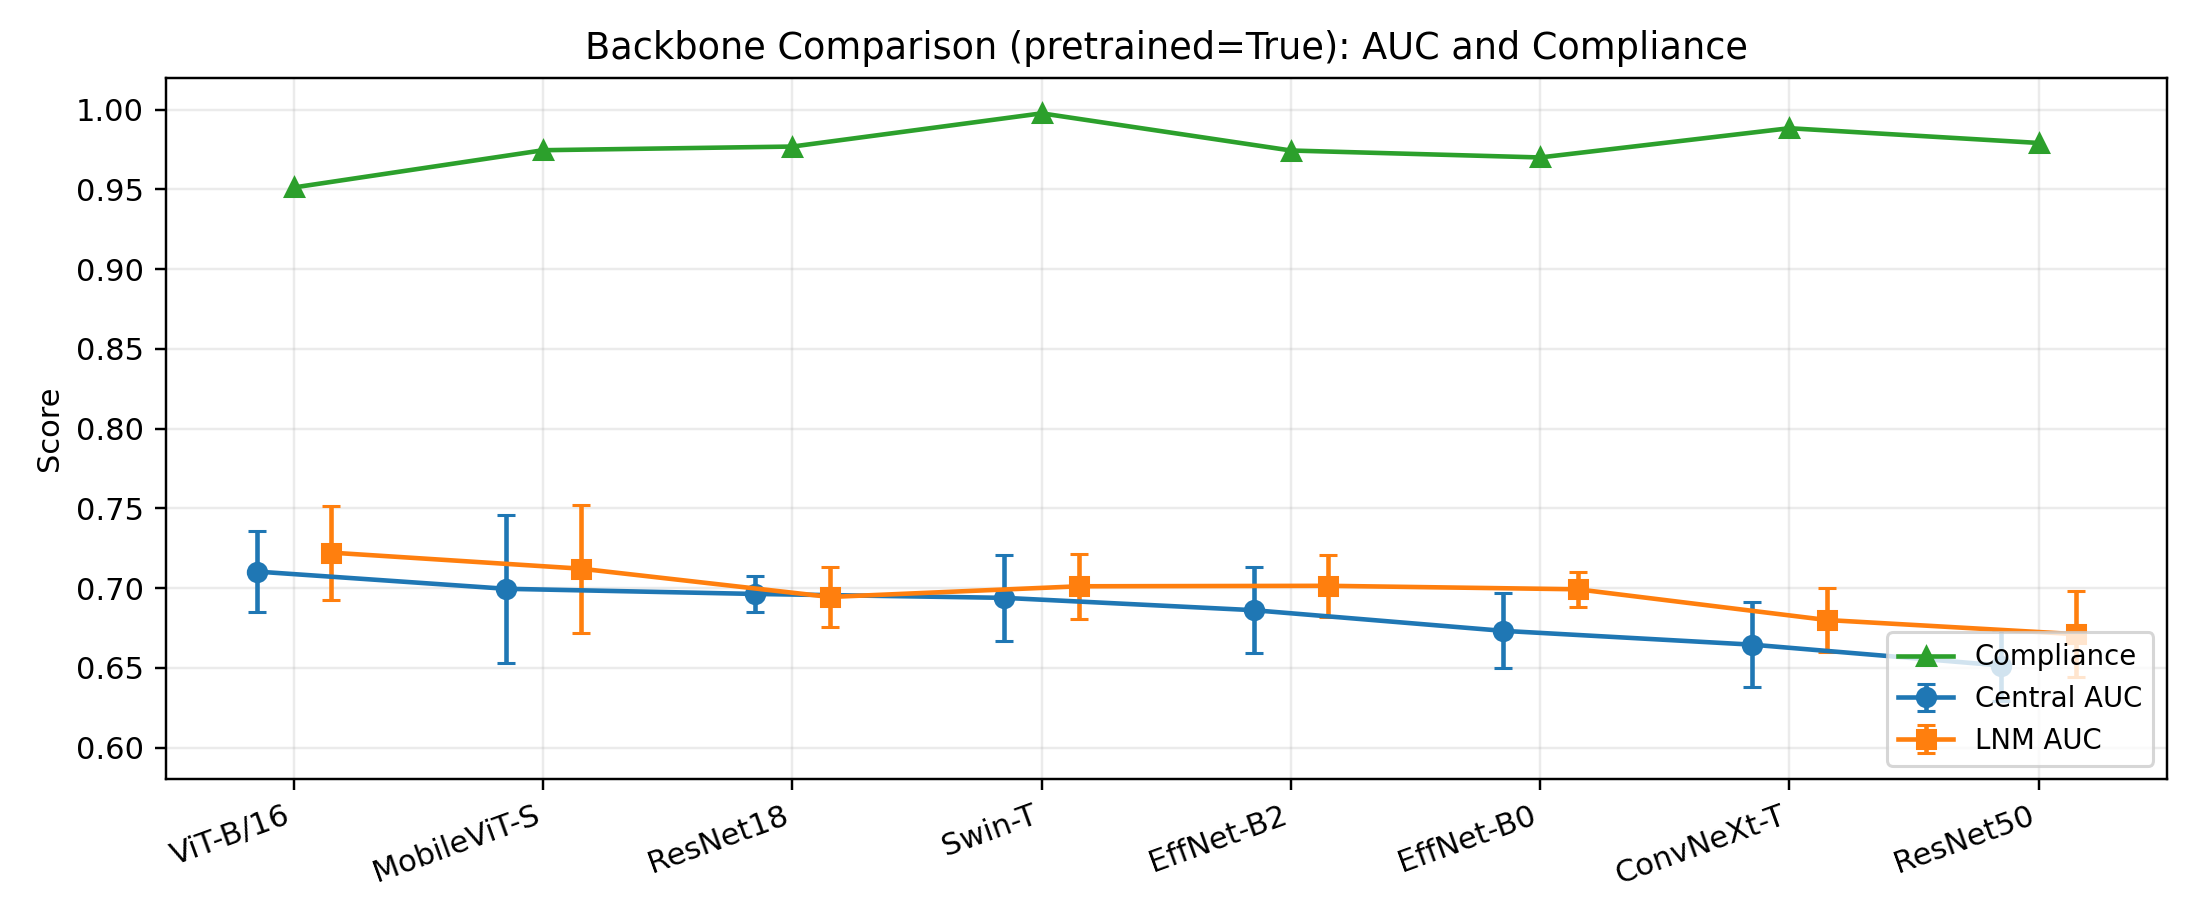
\includegraphics[width=0.9\textwidth]{figures/backbone_auc_compliance.png}
  \caption{8种骨干的 Central AUC、LNM AUC 与 Compliance 对比（误差线为5-fold std）。}
\end{figure}
\paragraph{结果解读}误差线显示 ViT-B/16 在 AUC 均值上领先，但 MobileViT-S 折间波动更大；Swin-T 虽 AUC 非最高，却在依从率上最稳定。
\paragraph{机制解释}启用预训练后，Transformer 家族在本任务上的表现较先前无预训练对比明显改善；但其稳定性仍依赖具体架构与参数规模，不宜简单概括为“Transformer 全面优于 CNN”。

\begin{figure}[H]
  \centering
  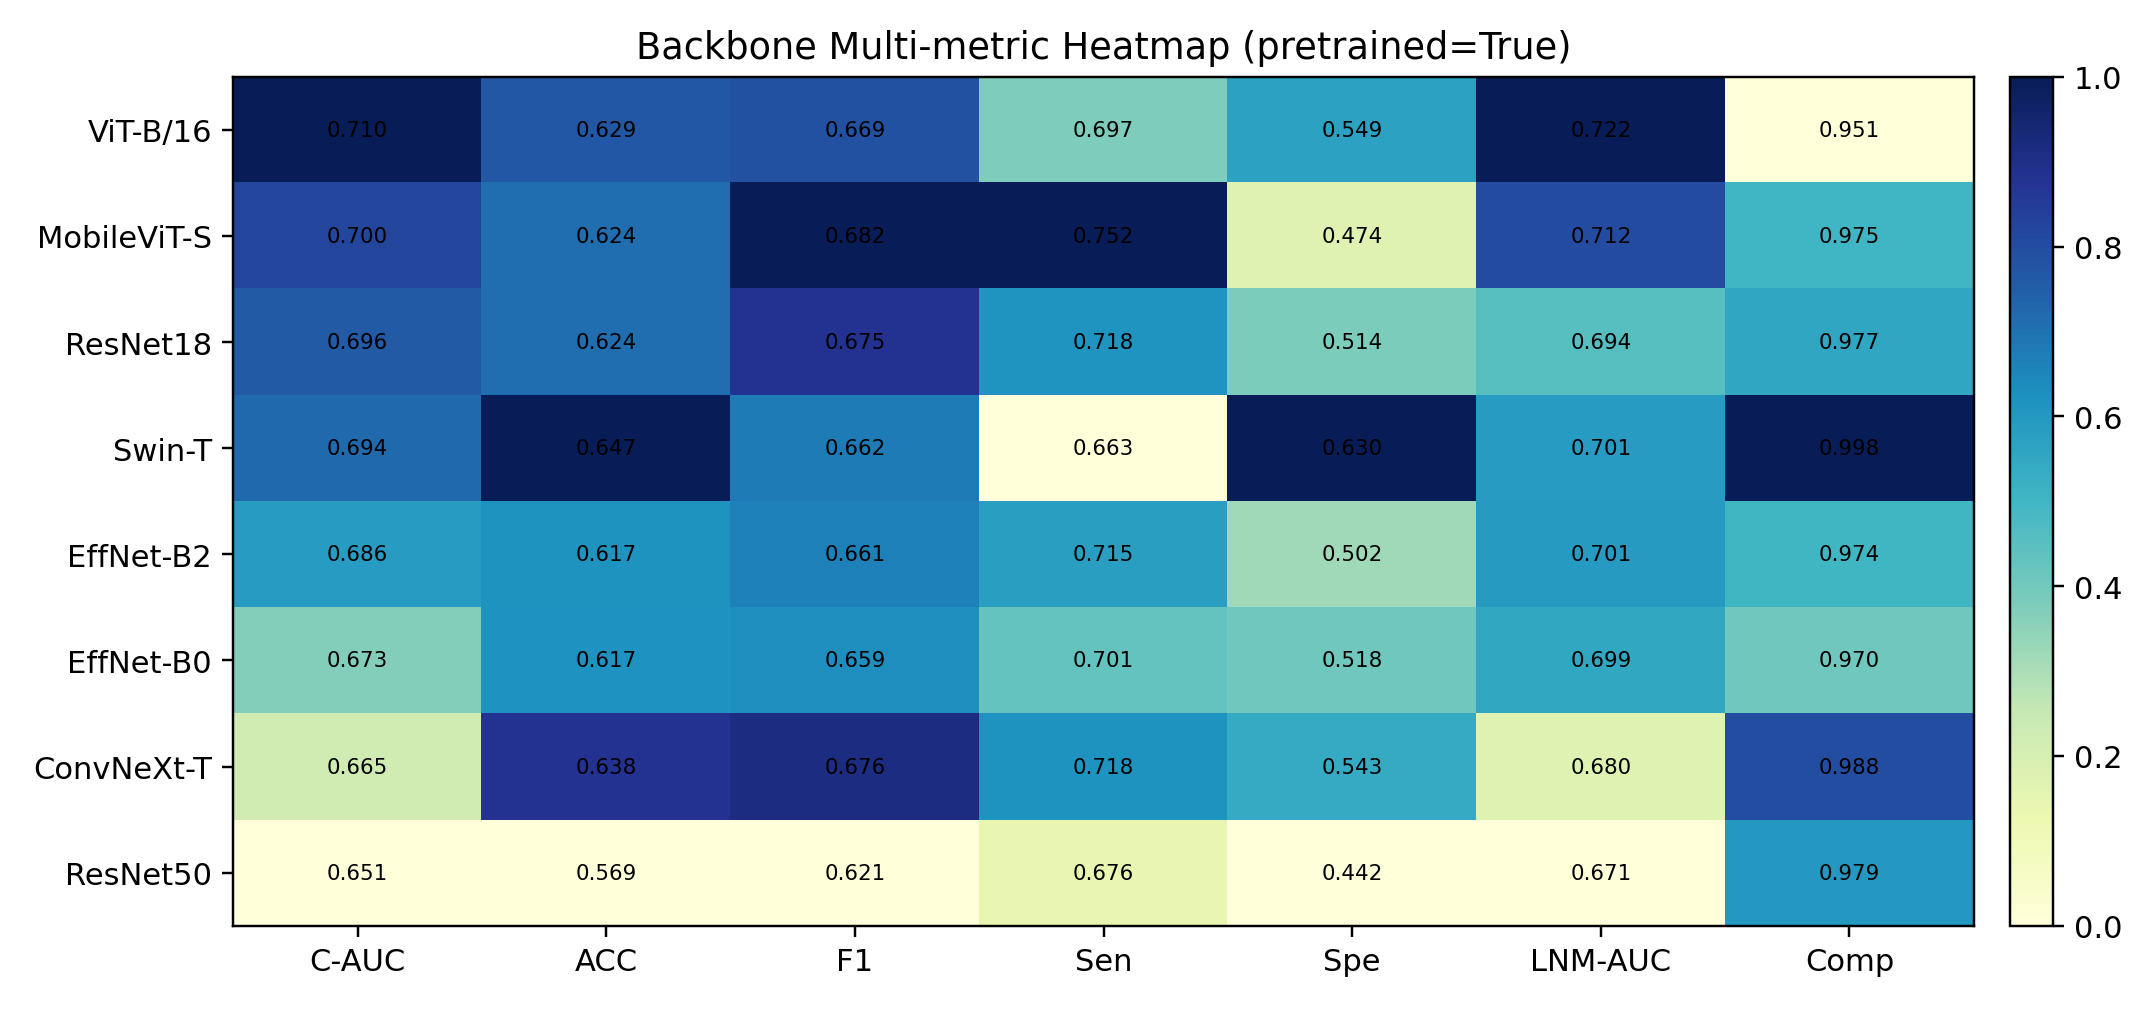
\includegraphics[width=0.9\textwidth]{figures/backbone_metrics_heatmap.png}
  \caption{8种骨干的多指标热力图（图中标注原始数值）。}
\end{figure}
\paragraph{关键观察}热力图提示不存在“所有指标同时最优”的单一骨干：不同模型分别在 AUC、Sensitivity、Specificity 与 Compliance 上占优，存在明确权衡关系。
\paragraph{模型选择策略}若以 AUC 作为主目标，ViT-B/16 为当前首选；若强调筛查灵敏度，可优先考虑 MobileViT-S；若强调临床规则一致性与特异度，Swin-T 更具优势。后续外部验证将按临床场景确定阈值与主评价指标。

\paragraph{一致性声明（表2 vs 表3）}
表2（6组消融）与表3（骨干公平对比）来自不同实验维度：前者强调模块消融最优组合，后者强调跨骨干统一协议可比性。ResNet18 在表3中直接复用了同协议历史结果（\texttt{pretrained=True}、freeze=3、5-fold），其余骨干为本轮同协议重跑；两表不做逐项等同比较，结论以同任务目标下的联合指标判读为准。

\subsection{三源融合续跑（ROI Radiomics + Deep MIL + Clinical Gated）}
在既有 6 组消融基础上，进一步完成“临床 + 深度 + 标准 ROI 组学”的系统续跑。流程分为三步：首先基于 B 模态原图与原始 mask 做 PyRadiomics，并在训练集内 LASSO 降维形成患者级组学向量；其次以 EffNet-B0 复现 Ours V1（Deep MIL + Clinical Gated，\texttt{pretrained=True}，前3个 epoch 冻结骨干后解冻）；最后在相同协议下加入组学分支得到 Ours V2（Tri-Fusion）。

\begin{table}[H]
\centering
\caption{三源续跑阶段核心结果（CentralLNM，5-fold test）}
\small
\begin{tabular}{lcccccc}
\toprule
设置 & AUC Mean$\pm$Std & ACC & F1 & Sen & Spe & Compliance \\
\midrule
C: Rad-only & 0.5756 $\pm$ 0.0538 & 0.5566 & 0.6151 & 0.6536 & 0.4417 & -- \\
D: Clin+Rad & \textbf{0.6923 $\pm$ 0.0696} & 0.6330 & 0.6672 & 0.6839 & \textbf{0.5729} & -- \\
V1: Deep+Clin (EffB0) & 0.6732 $\pm$ 0.0236 & 0.6173 & 0.6592 & 0.7014 & 0.5178 & \textbf{0.9700 $\pm$ 0.0382} \\
V2: Tri-Fusion (EffB0) & 0.6708 $\pm$ 0.0544 & \textbf{0.6426} & \textbf{0.6826} & \textbf{0.7096} & 0.5632 & 0.9603 $\pm$ 0.0311 \\
\bottomrule
\end{tabular}
\end{table}
\paragraph{缩写说明}C=ROI Radiomics-only（LogReg）；D=Clinical+ROI Radiomics（SoftVoting）；V1=Deep MIL + Clinical Gated；V2=Tri-Fusion（Deep+Clinical+ROI Radiomics）。
\paragraph{结果解读}ROI 组学单独建模仍偏弱，但与临床拼接后（Baseline D）可达到较高 AUC；说明组学对临床具有补充价值。
\paragraph{结果解读}三源门控（Ours V2）在 ACC/F1/Sen/Spe 上更均衡，但 AUC 未超过 Ours V1，提示当前“组学-深度交互”仍有优化空间。

\begin{figure}[H]
  \centering
  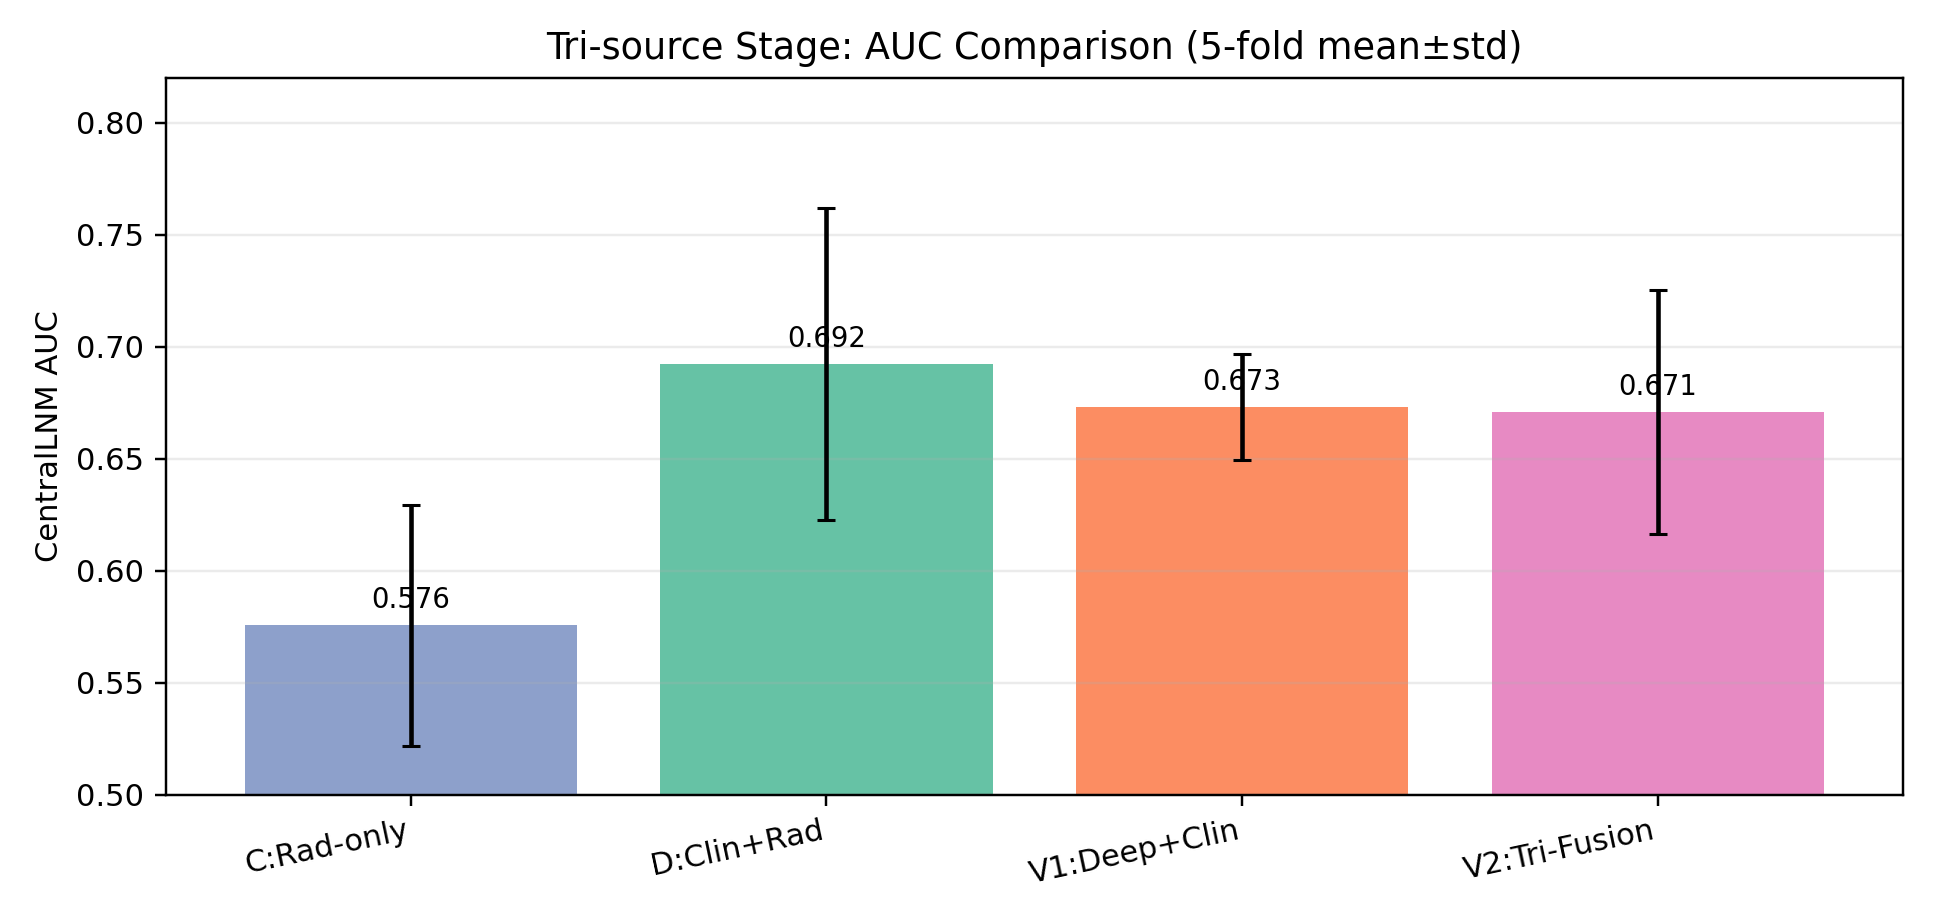
\includegraphics[width=0.82\textwidth]{figures/tri_source_auc_compare.png}
  \caption{三源续跑阶段 4 组设置的 CentralLNM AUC 对比（5-fold mean$\pm$std）。}
\end{figure}
\paragraph{图表分析}AUC 结果显示 D 组均值最高，但标准差也较大，提示其在不同折次存在一定不稳定性。
\paragraph{图表分析}V1/V2 在 AUC 上接近，说明当前三源增益并非体现在单一 AUC 指标的显著提升，而更可能体现在多指标平衡。

\begin{figure}[H]
  \centering
  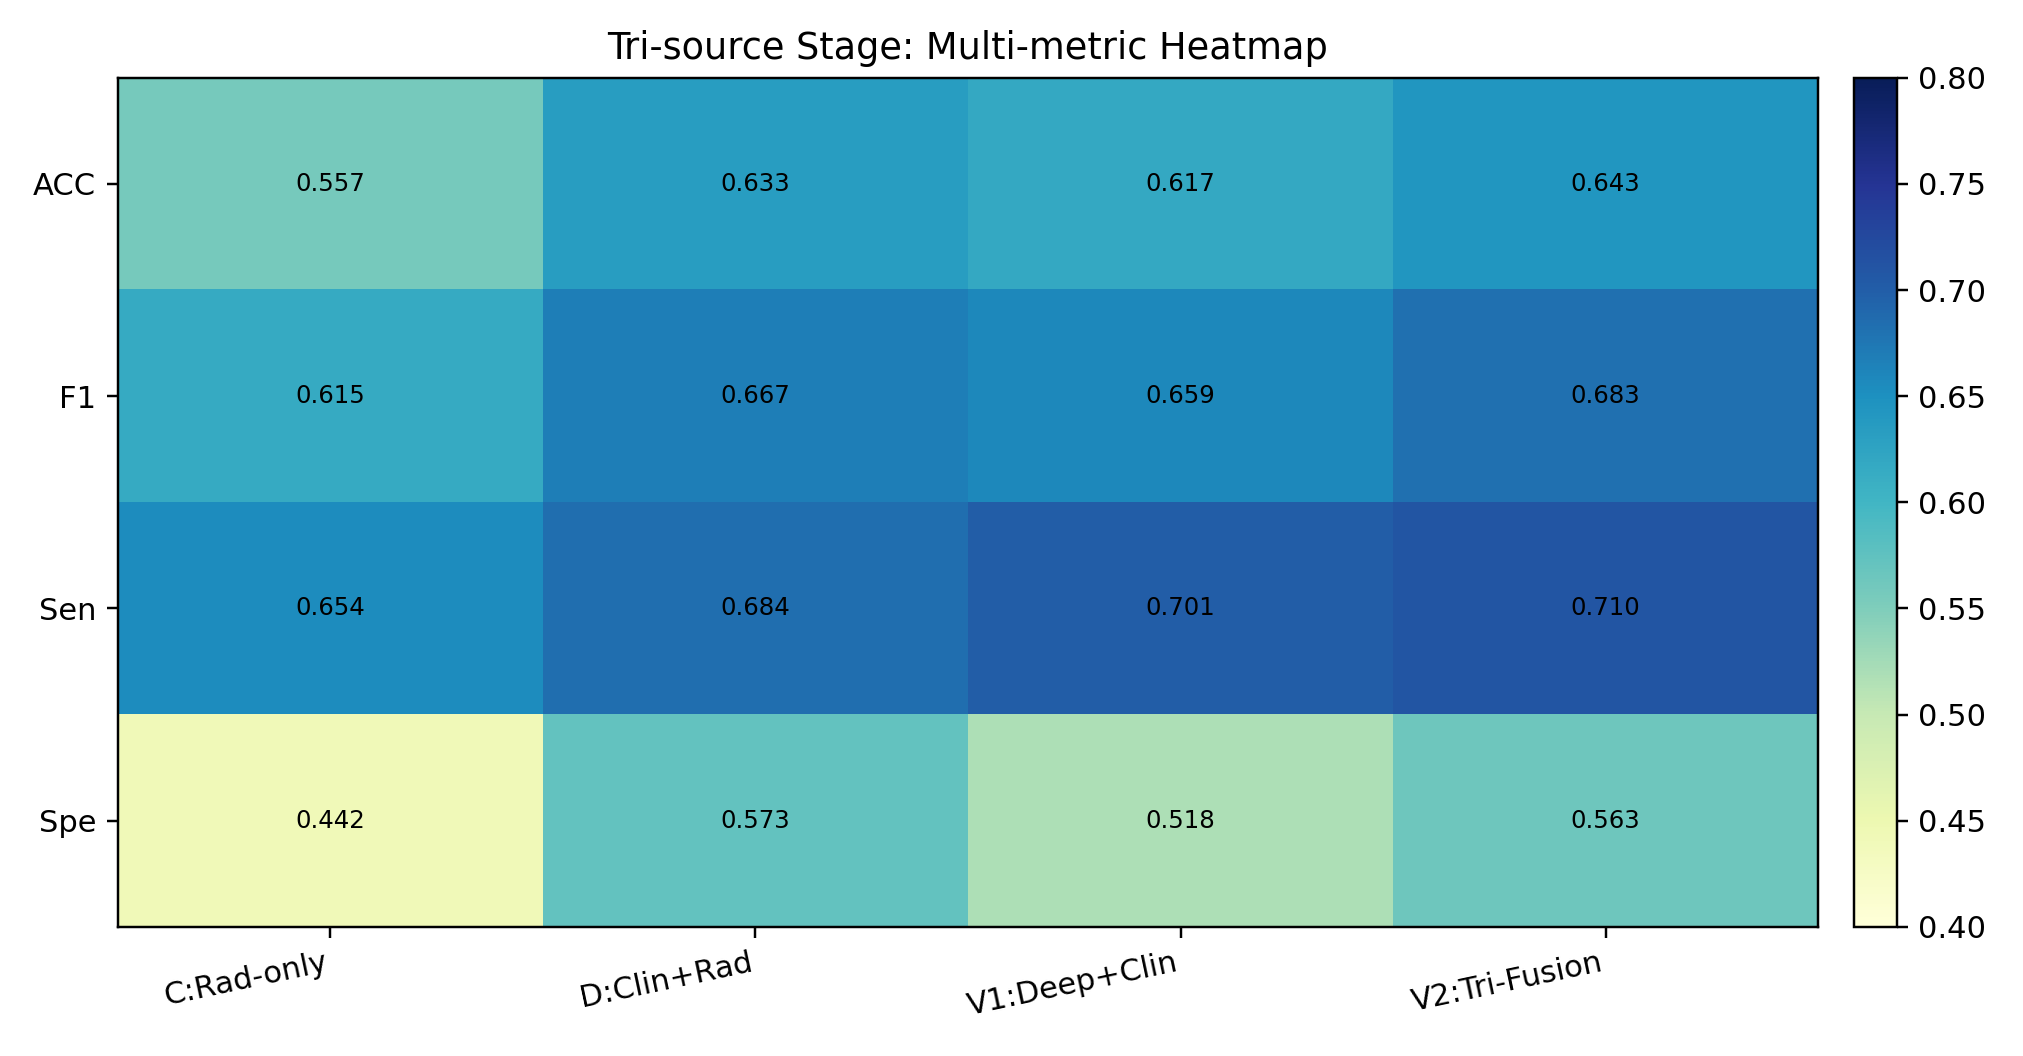
\includegraphics[width=0.82\textwidth]{figures/tri_source_metrics_heatmap.png}
  \caption{三源续跑阶段多指标热力图（ACC/F1/Sen/Spe）。}
\end{figure}
\paragraph{图表分析}热力图可见 V2 在 ACC/F1/Sen 上整体优于 V1，且 Spe 也较 C 组有明显改善，体现“融合后判别更均衡”的特征。
\paragraph{图表分析}D 组在 AUC 领先但敏感度提升有限，提示传统融合对排序能力有帮助，而深度三源在阈值相关指标上仍有进一步优化空间。

\subsection{三源融合多版本对比（V1 + 三个版本V2）}
为回答“V2退化是否由融合方式造成”，在相同数据划分与训练协议下，进一步比较：
V1（Deep+Clin）与三种 V2（legacy / align\_proj / FiLM），并在 EffB0、Swin-T、ViT-B/16 三个骨干上统一报告多指标。

\begin{table}[H]
\centering
\caption{EffB0：V1 与三版本 V2 对比（5-fold test）}
\small
\begin{tabular}{lccccccc}
\toprule
版本 & AUC$_{cen}$ & AUC$_{lnm}$ & ACC & F1 & Sen & Spe & Compliance \\
\midrule
V1 & 0.6732$\pm$0.0236 & 0.6992$\pm$0.0110 & 0.6173 & 0.6592 & 0.7014 & 0.5178 & 0.9700$\pm$0.0382 \\
V2-legacy & 0.6708$\pm$0.0544 & 0.7032$\pm$0.0388 & 0.6426 & 0.6826 & 0.7096 & 0.5632 & 0.9603$\pm$0.0311 \\
V2-align\_proj & 0.6911$\pm$0.0323 & 0.7037$\pm$0.0257 & 0.6034 & 0.6228 & 0.6290 & \textbf{0.5744} & 0.9608$\pm$0.0408 \\
V2-FiLM & \textbf{0.6951$\pm$0.0354} & 0.6978$\pm$0.0323 & 0.6333 & \textbf{0.6930} & \textbf{0.7607} & 0.4826 & \textbf{0.9747$\pm$0.0303} \\
\bottomrule
\end{tabular}
\end{table}

\begin{table}[H]
\centering
\caption{Swin-T：V1 与三版本 V2 对比（5-fold test）}
\small
\begin{tabular}{lccccccc}
\toprule
版本 & AUC$_{cen}$ & AUC$_{lnm}$ & ACC & F1 & Sen & Spe & Compliance \\
\midrule
V1 & \textbf{0.6939$\pm$0.0267} & \textbf{0.7011$\pm$0.0203} & \textbf{0.6473} & \textbf{0.6620} & 0.6635 & \textbf{0.6296} & \textbf{0.9977$\pm$0.0047} \\
V2-legacy & 0.6793$\pm$0.0313 & 0.6914$\pm$0.0343 & 0.6263 & 0.6601 & \textbf{0.6709} & 0.5736 & 0.9348$\pm$0.0853 \\
V2-align\_proj & 0.6646$\pm$0.0434 & \textbf{0.7015$\pm$0.0453} & 0.5942 & 0.6264 & 0.6325 & 0.5499 & 0.9723$\pm$0.0237 \\
V2-FiLM & 0.6631$\pm$0.0399 & 0.6679$\pm$0.0326 & 0.6009 & 0.6278 & 0.6424 & 0.5514 & 0.9724$\pm$0.0440 \\
\bottomrule
\end{tabular}
\end{table}

\begin{table}[H]
\centering
\caption{ViT-B/16：V1 与三版本 V2 对比（5-fold test）}
\small
\begin{tabular}{lccccccc}
\toprule
版本 & AUC$_{cen}$ & AUC$_{lnm}$ & ACC & F1 & Sen & Spe & Compliance \\
\midrule
V1 & \textbf{0.7104$\pm$0.0253} & \textbf{0.7222$\pm$0.0295} & 0.6289 & 0.6686 & 0.6969 & 0.5490 & 0.9512$\pm$0.0626 \\
V2-legacy & 0.6404$\pm$0.0496 & 0.6592$\pm$0.0522 & 0.5779 & 0.6478 & \textbf{0.7220} & 0.4077 & 0.9398$\pm$0.0621 \\
V2-align\_proj & 0.6971$\pm$0.0356 & 0.7155$\pm$0.0217 & 0.6403 & 0.6505 & 0.6327 & \textbf{0.6495} & 0.9561$\pm$0.0601 \\
V2-FiLM & 0.6868$\pm$0.0451 & 0.6991$\pm$0.0451 & \textbf{0.6428} & \textbf{0.6706} & 0.6663 & 0.6149 & \textbf{0.9837$\pm$0.0158} \\
\bottomrule
\end{tabular}
\end{table}

\begin{figure}[H]
  \centering
  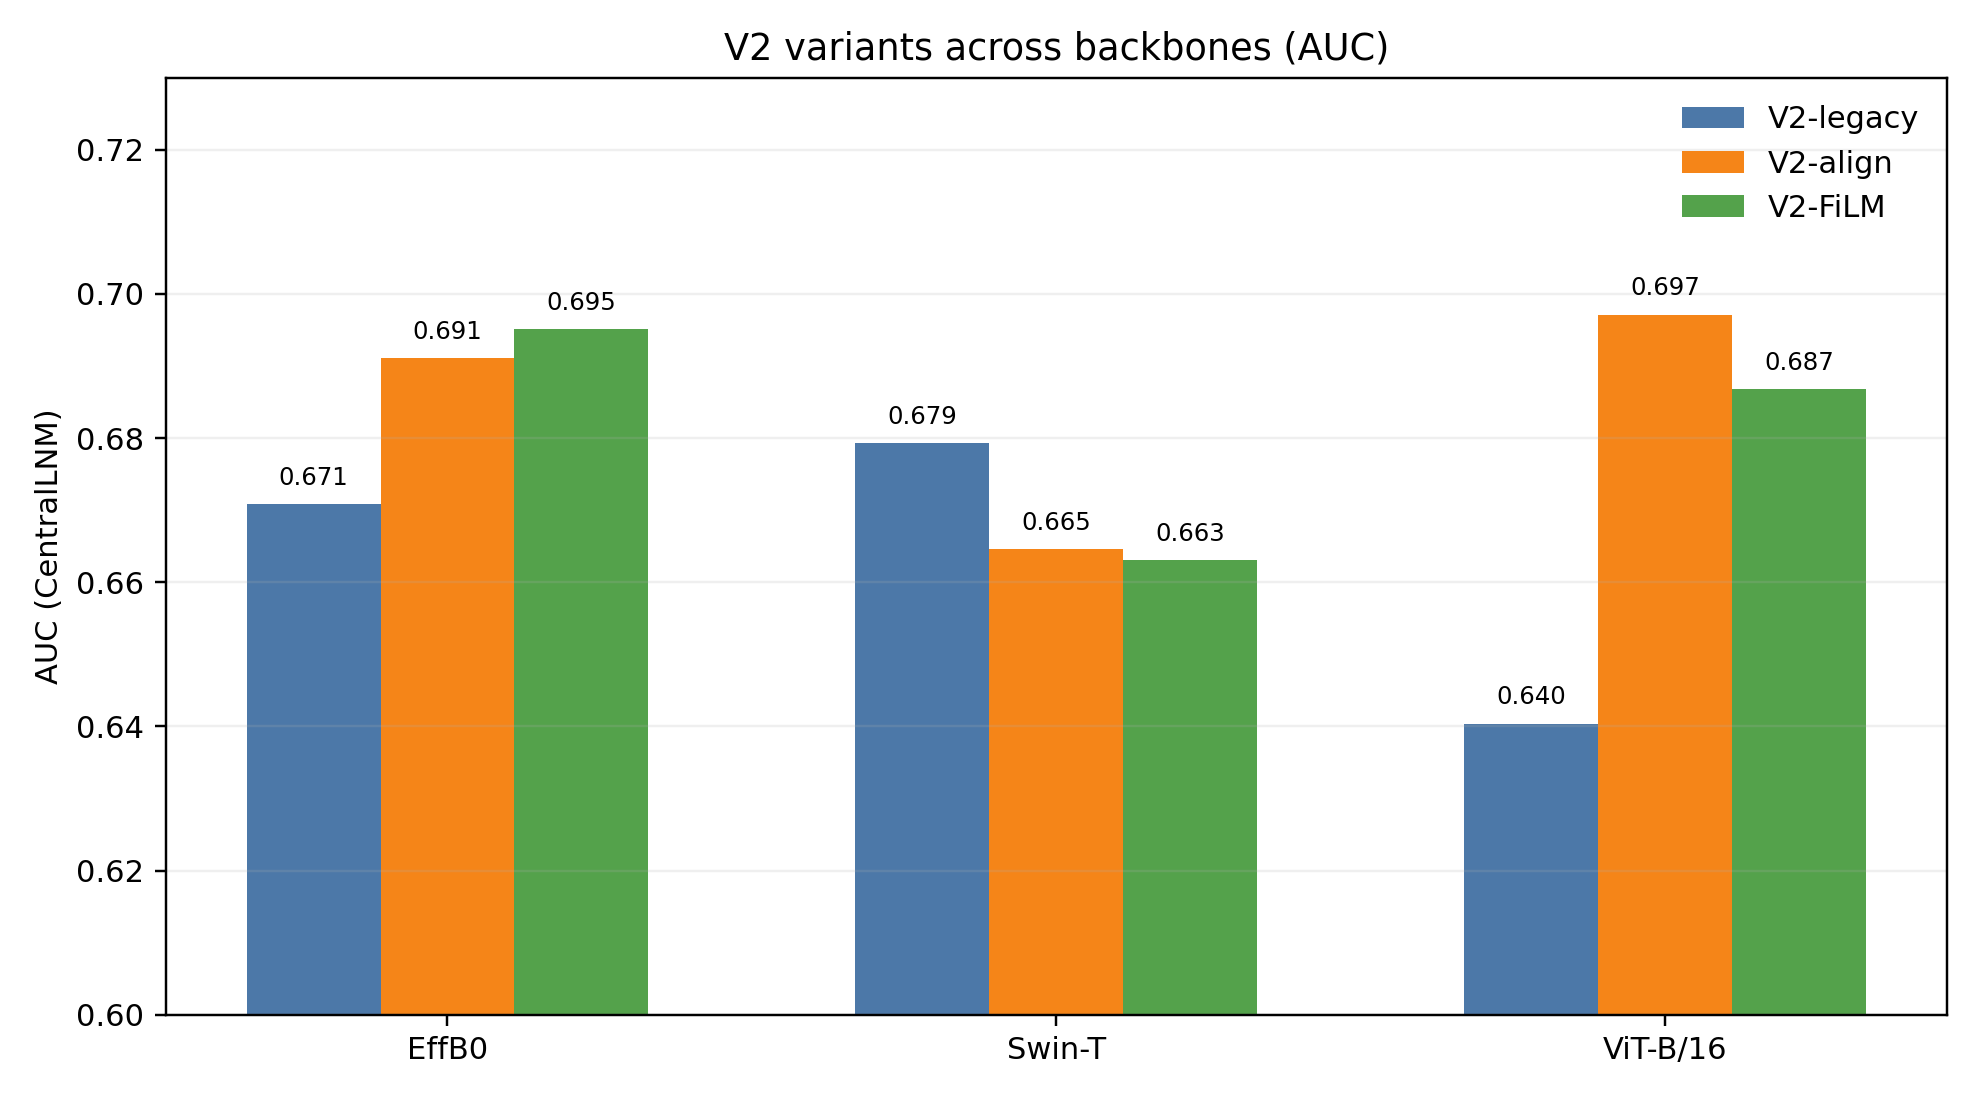
\includegraphics[width=0.86\textwidth]{figures/v2_versions_auc_grouped.png}
  \caption{三骨干在三种 V2 融合策略（legacy / align\_proj / FiLM）下的 CentralLNM AUC 对比。}
\end{figure}
\paragraph{图表分析}AUC 柱状图显示：EffB0 在 FiLM 下达到当前最高；ViT 在 align\_proj 下提升最明显；Swin 在当前两种新融合器下均未超过 legacy。

\begin{figure}[H]
  \centering
  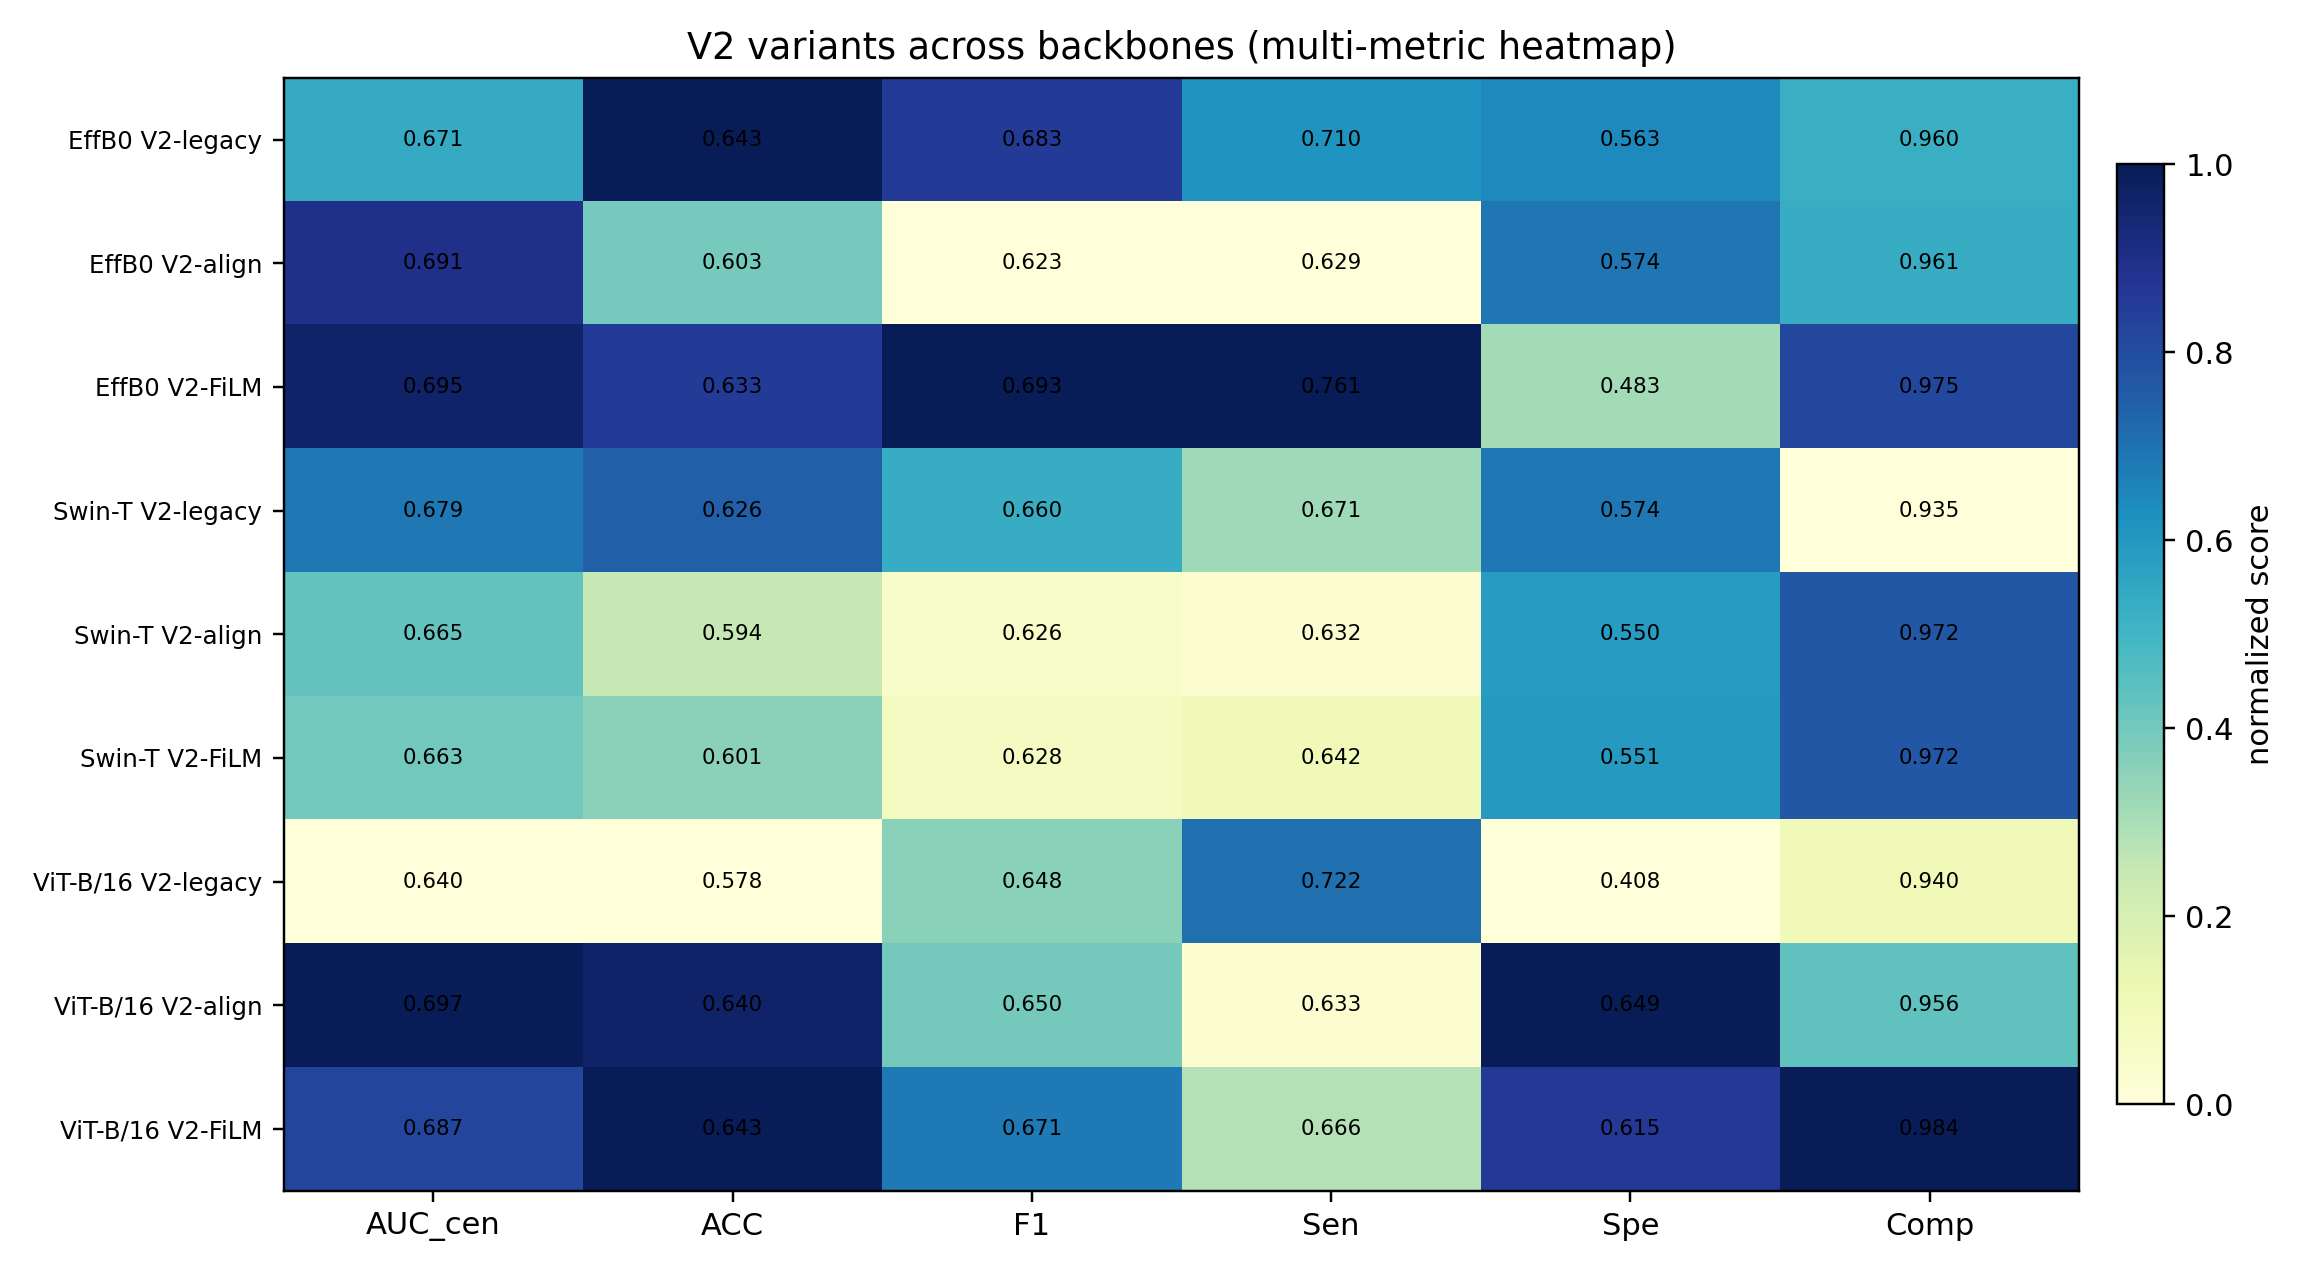
\includegraphics[width=0.94\textwidth]{figures/v2_versions_metrics_heatmap.png}
  \caption{三骨干-三策略的多指标热力图（列内归一化着色，格内为原始数值）。}
\end{figure}
\paragraph{图表分析}热力图进一步表明“同一融合器难以跨骨干统一最优”：FiLM 更偏向提升 EffB0 的召回与综合分数，align\_proj 更有利于 ViT 的排序能力与特异度，而 Swin 仍更依赖原始融合范式。

\begin{figure}[H]
  \centering
  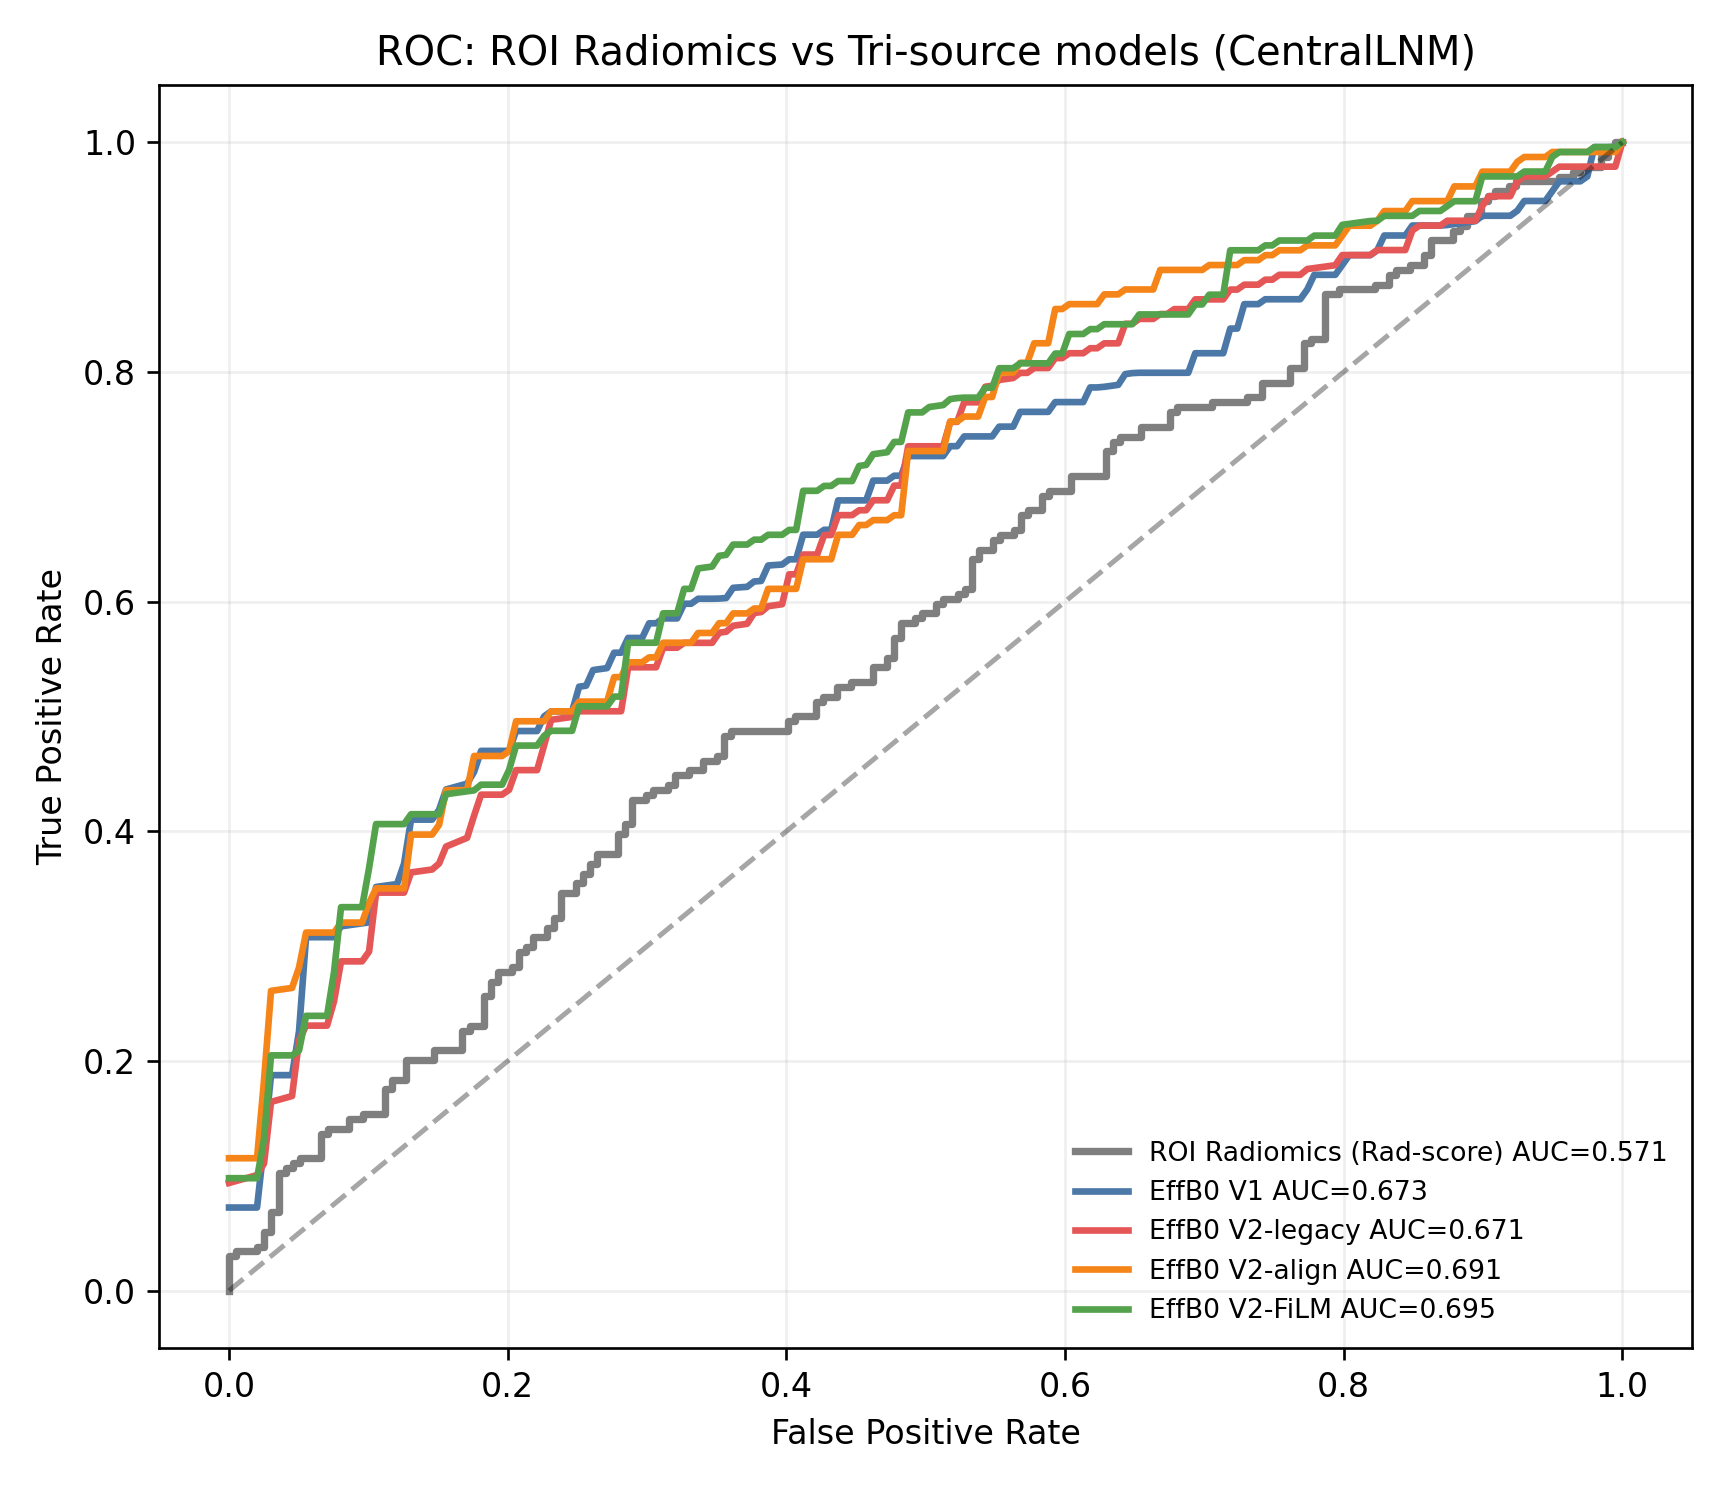
\includegraphics[width=0.82\textwidth]{figures/roi_radiomics_vs_tri_source_roc.png}
  \caption{ROI Radiomics（患者级 Rad-score）与 EffB0 三源模型的 ROC 对比（CentralLNM）。}
\end{figure}
\paragraph{图表分析}影像组学分支（Rad-score）可提供独立可解释信号，但单独 ROC 表现低于三源深度融合；在引入对齐或调制后，三源模型曲线整体上移，说明组学信息在合理融合下可转化为稳健增益而非噪声。

\paragraph{关键差值分析（AUC$_{cen}$）}
\begin{itemize}
  \item EffB0：legacy 相比 V1 近似持平（$-0.0024$），align\_proj 与 FiLM 分别提升 $+0.0203$、$+0.0243$，FiLM 最优。
  \item Swin-T：legacy 相比 V1 降低 $0.0146$，align\_proj 与 FiLM 进一步下降（$-0.0147$、$-0.0162$），说明该骨干当前对新融合器不敏感或需专门调参。
  \item ViT-B/16：legacy 相比 V1 明显下降（$-0.0700$）；align\_proj 与 FiLM 相比 legacy 显著恢复（$+0.0567$、$+0.0464$），其中 align\_proj 的 AUC 恢复最好，FiLM 的一致性（Compliance）最佳。
\end{itemize}

\paragraph{决策建议}
\begin{itemize}
  \item 以 AUC 为主：EffB0 选 FiLM，ViT 选 align\_proj，Swin 暂保留 legacy。
  \item 以临床一致性（Compliance）与阈值稳健性（Spe）为主：ViT 可优先 FiLM；EffB0 也可优先 FiLM；Swin 维持 V1 或 legacy 作为稳健版本。
  \item 不建议“单一融合器跨骨干统一部署”；更合理的是骨干特异策略（backbone-specific fusion）。
\end{itemize}

\subsection{原始临床回归基线结果}
在原始临床变量基础上，进一步完成三任务（LNM / CentralLNM / LateralLNM）的经典 Logistic 回归基线。与深度模型一致，仍使用患者级 5-fold 划分；不同之处在于该基线不依赖预处理 `clinical_features.csv`，而是直接从原始 Excel 的术前变量建模。

\begin{table}[H]
\centering
\caption{原始临床回归基线结果（5-fold test）}
\small
\begin{tabular}{lccccc}
\toprule
任务 & AUC Mean$\pm$Std & ACC & F1 & Sen & Spe \\
\midrule
LNM & 0.7023$\pm$0.0448 & 0.6356 & 0.6705 & 0.6721 & 0.5880 \\
CentralLNM & 0.6859$\pm$0.0658 & 0.6332 & 0.6661 & 0.6712 & 0.5881 \\
LateralLNM & 0.8409$\pm$0.0902 & 0.9094 & 0.3055 & 0.2818 & 0.9720 \\
\bottomrule
\end{tabular}
\end{table}

\begin{figure}[H]
  \centering
  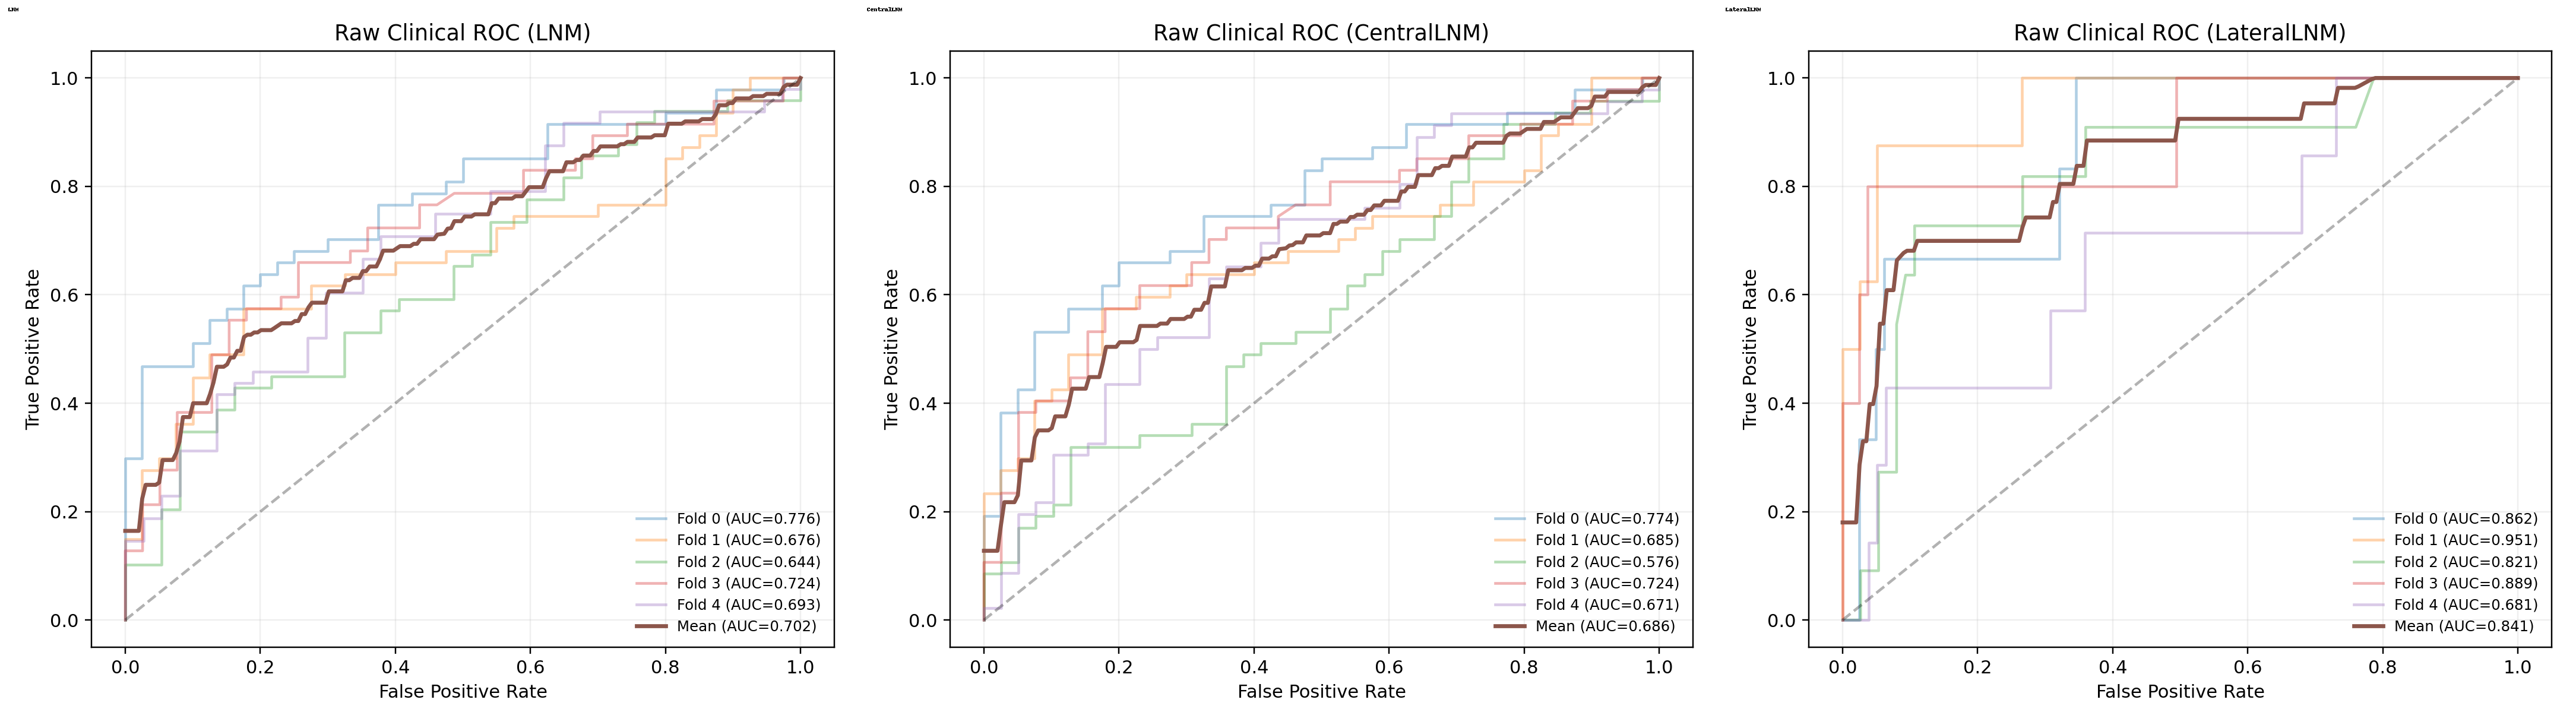
\includegraphics[width=0.96\textwidth]{figures/raw_clinical_roc_panel.png}
  \caption{原始临床回归基线在 LNM、CentralLNM 与 LateralLNM 三任务上的 ROC 曲线。}
\end{figure}
\paragraph{结果解读}原始临床回归基线在 `CentralLNM` 上获得约 0.686 的 AUC，说明即使不借助深度影像特征，仅凭术前临床变量也已有较强判别能力；这使其成为论文中更合理的临床参照。`LNM` 任务的 AUC 进一步达到约 0.702，提示整体转移状态与术前临床变量的关联更稳定。`LateralLNM` 虽然 AUC 较高，但灵敏度明显偏低而特异度极高，说明该任务在当前基线下更倾向保守判阳，因此不应仅用 AUC 单指标评价其临床实用性。

\begin{table}[H]
\centering
\caption{单因素筛选中最稳定的特征（$p<0.05$，5-fold 频次）}
\small
\begin{tabular}{lccc}
\toprule
特征 & LNM & CentralLNM & LateralLNM \\
\midrule
超声探及淋巴结异常（1=中央VI区） & 5/5 & 4/5 & 5/5 \\
超声探及淋巴结异常（2=侧方） & 1/5 & 1/5 & 5/5 \\
calcification（micro） & 5/5 & 5/5 & 0/5 \\
年龄 & 5/5 & 5/5 & 2/5 \\
size（前后径）cm & 4/5 & 4/5 & 3/5 \\
size（长径/横径）cm & 4--5/5 & 4/5 & 0/5 \\
性别（男） & 3/5 & 4/5 & 3/5 \\
\bottomrule
\end{tabular}
\end{table}

\begin{table}[H]
\centering
\caption{多因素模型中跨折最稳定的入选特征（按入选频次与中位 OR）}
\small
\begin{tabular}{p{0.44\textwidth}ccc}
\toprule
特征（one-hot 展开后） & LNM & CentralLNM & LateralLNM \\
\midrule
超声探及淋巴结异常（1=中央VI区） & 5/5，OR$\approx$6.41 & 5/5，OR$\approx$4.03 & 5/5，OR$\approx$17.45 \\
超声探及淋巴结异常（2=侧方） & 1/5，OR$\approx$5.38 & 1/5，OR$\approx$5.25 & 5/5，OR$\approx$46.19 \\
calcification（micro） & 5/5，OR$\approx$2.05 & 5/5，OR$\approx$2.09 & 2/5，OR$\approx$3.11 \\
年龄（每增1岁） & 5/5，OR$\approx$0.95 & 5/5，OR$\approx$0.96 & 3/5，OR$\approx$0.97 \\
size（前后径）cm & 4/5，OR$\approx$1.87 & 4/5，OR$\approx$2.12 & 3/5，OR$\approx$7.88 \\
性别（男） & 5/5，OR$\approx$1.75 & 4/5，OR$\approx$1.67 & 4/5，OR$\approx$2.61 \\
多灶（多灶=1） & -- & -- & 3/5，OR$\approx$2.97 \\
\bottomrule
\end{tabular}
\end{table}

\paragraph{进一步解释}从单因素与多因素结果可见，三任务中最稳定的共同信号是“超声探及淋巴结异常”“微钙化”“年龄”与“结节尺寸”；其中 `LateralLNM` 对“侧方异常（=2）”的效应最强（跨折中位 OR 约 46），但该任务阳性样本较少，导致阈值相关指标（尤其灵敏度）在不同 fold 波动更明显。相对而言，`LNM/CentralLNM` 的入选特征更一致，提示其临床基线可解释性与稳定性更高。

\section{可解释性与临床决策评估}
\subsection{代表性病例：多切面 Grad-CAM（3例）}
按模型预测概率从测试集中自动选取高风险/中风险/低风险三类代表病例，并在图中角标标注 \texttt{PID / y / p\_central}：
\begin{figure}[H]
  \centering
  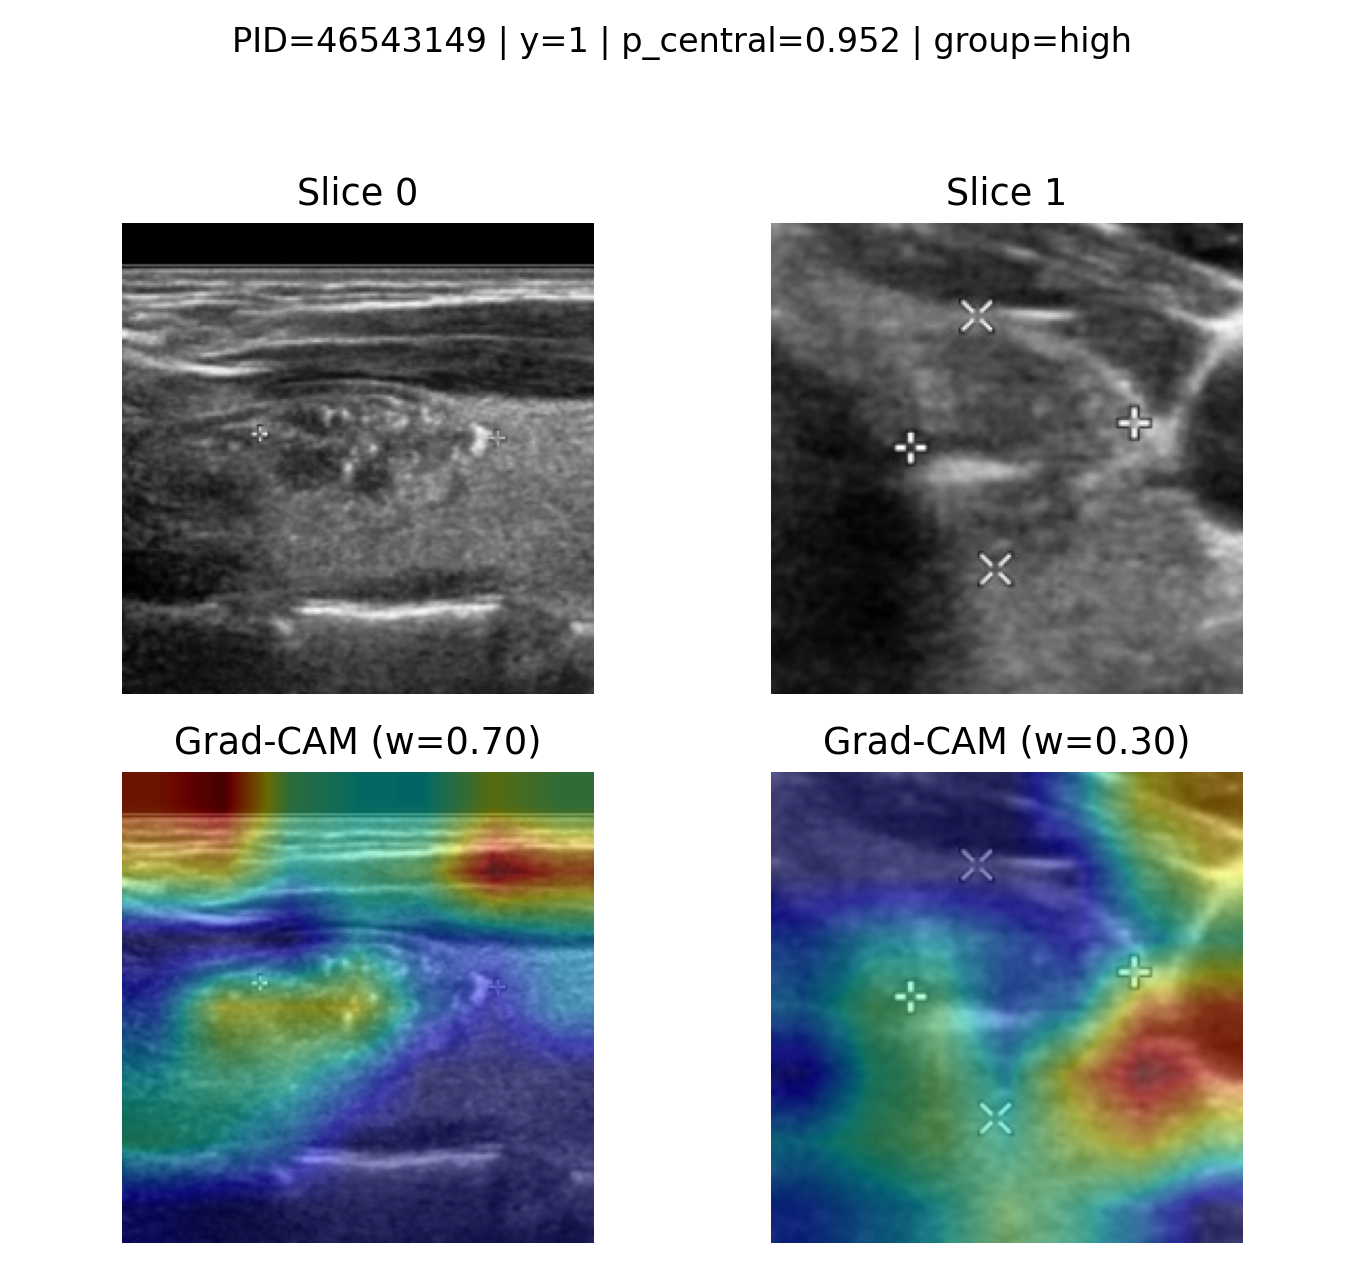
\includegraphics[width=0.92\textwidth]{figures/gradcam_slices_case_high.png}
  \caption{高风险代表病例（多切面 Grad-CAM）。}
\end{figure}
\paragraph{图表分析}该病例中 Top-attended 切面的激活区域更集中，且与高预测概率一致，提示模型在该病例存在较强判别证据链。

\begin{figure}[H]
  \centering
  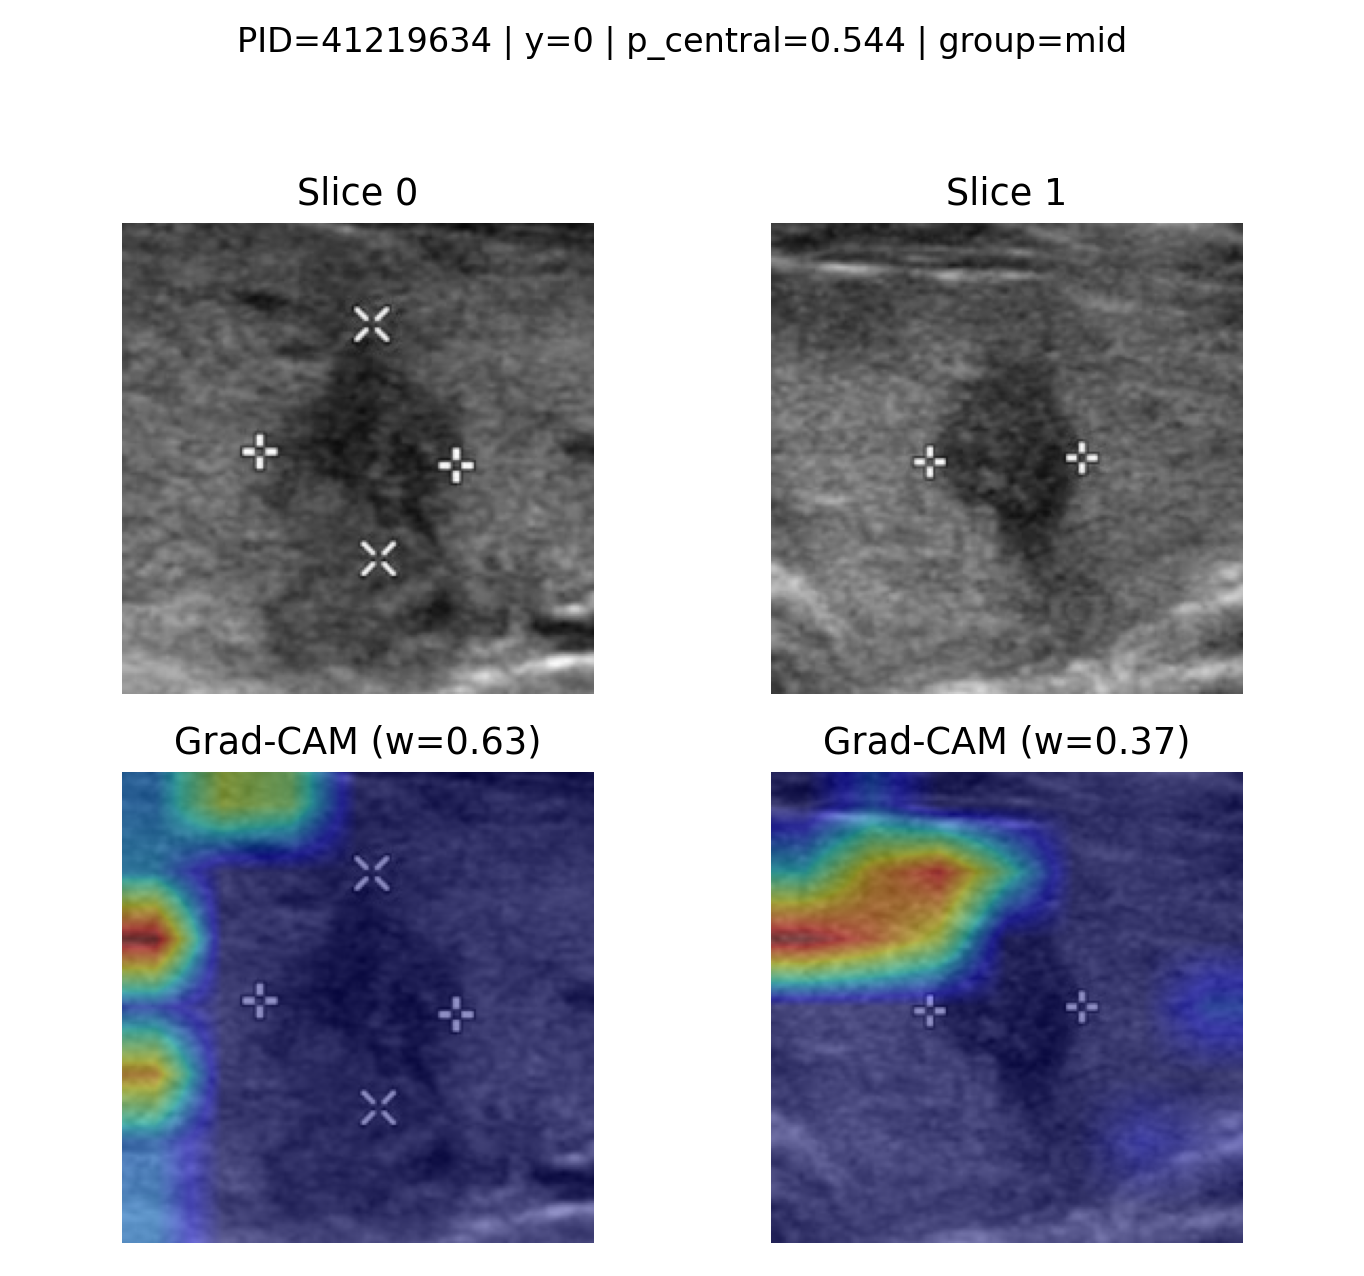
\includegraphics[width=0.92\textwidth]{figures/gradcam_slices_case_mid.png}
  \caption{中风险代表病例（多切面 Grad-CAM）。}
\end{figure}
\paragraph{图表分析}中风险病例的切面间激活强度差异更明显，显示模型在“可疑但不确定”状态下依赖少数关键切面做出判断。

\begin{figure}[H]
  \centering
  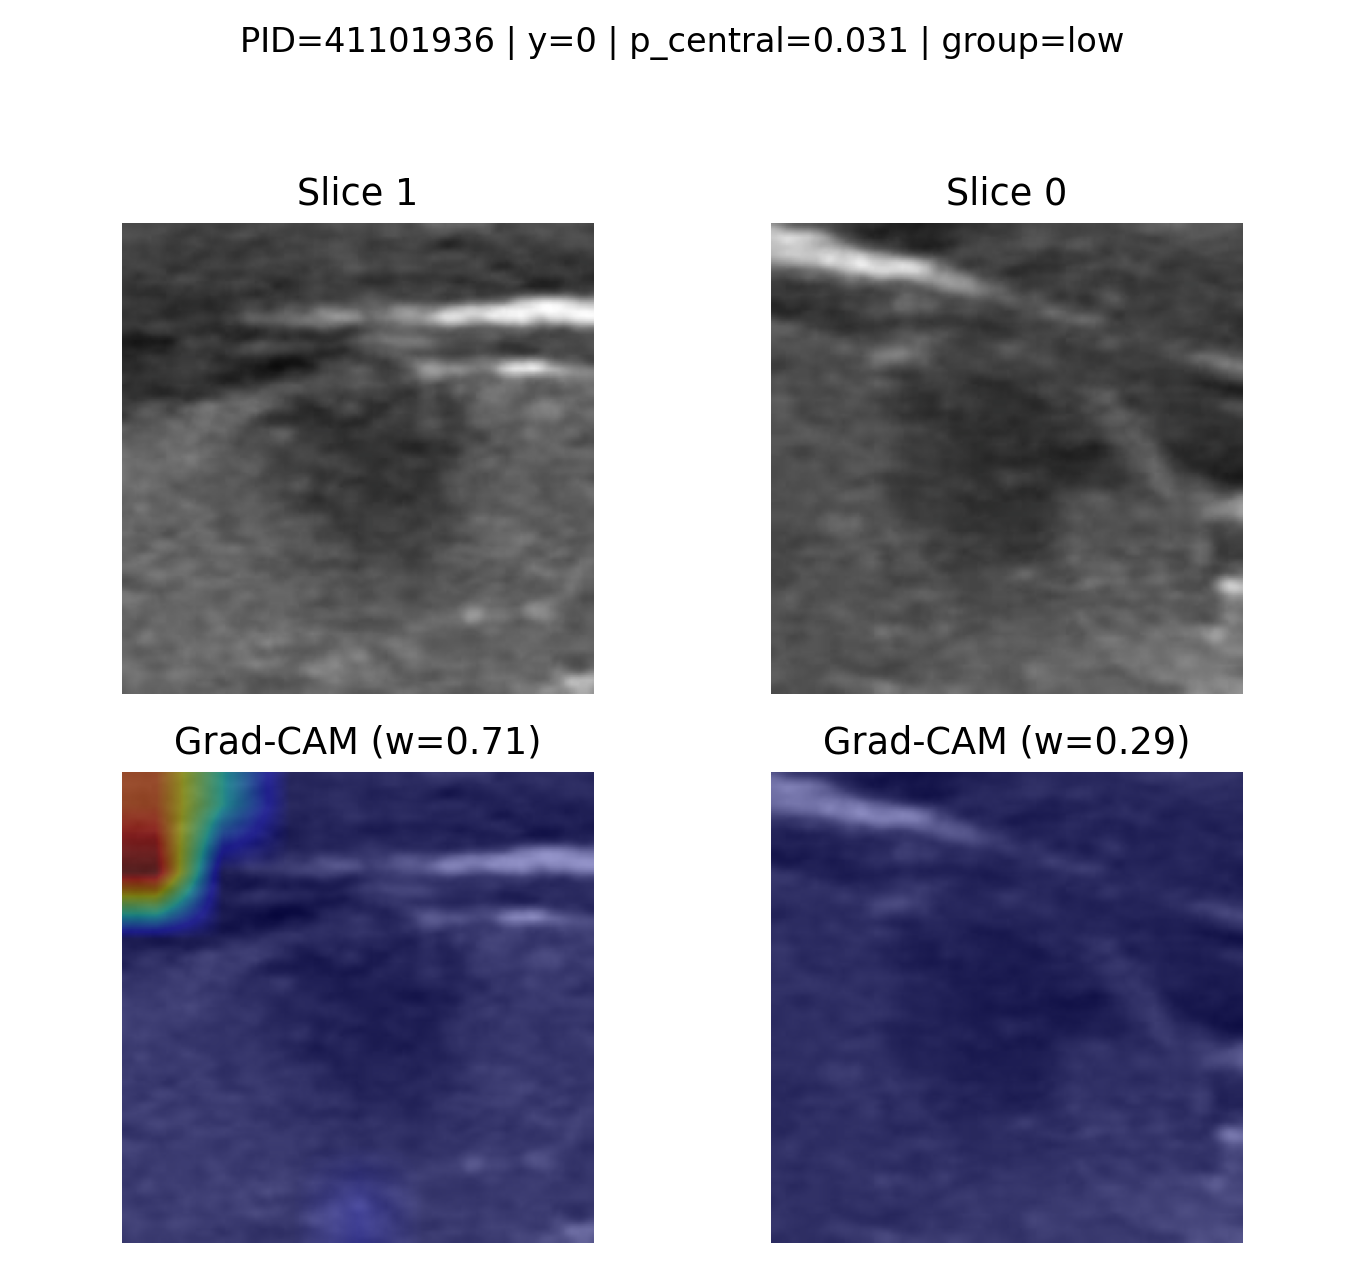
\includegraphics[width=0.92\textwidth]{figures/gradcam_slices_case_low.png}
  \caption{低风险代表病例（多切面 Grad-CAM）。}
\end{figure}
\paragraph{图表分析}低风险病例中激活区域更分散且整体响应较弱，与较低预测概率一致，支持模型对阴性样本的保守判别模式。

\subsection{代表性病例：多模态 Grad-CAM（3例）}
\begin{figure}[H]
  \centering
  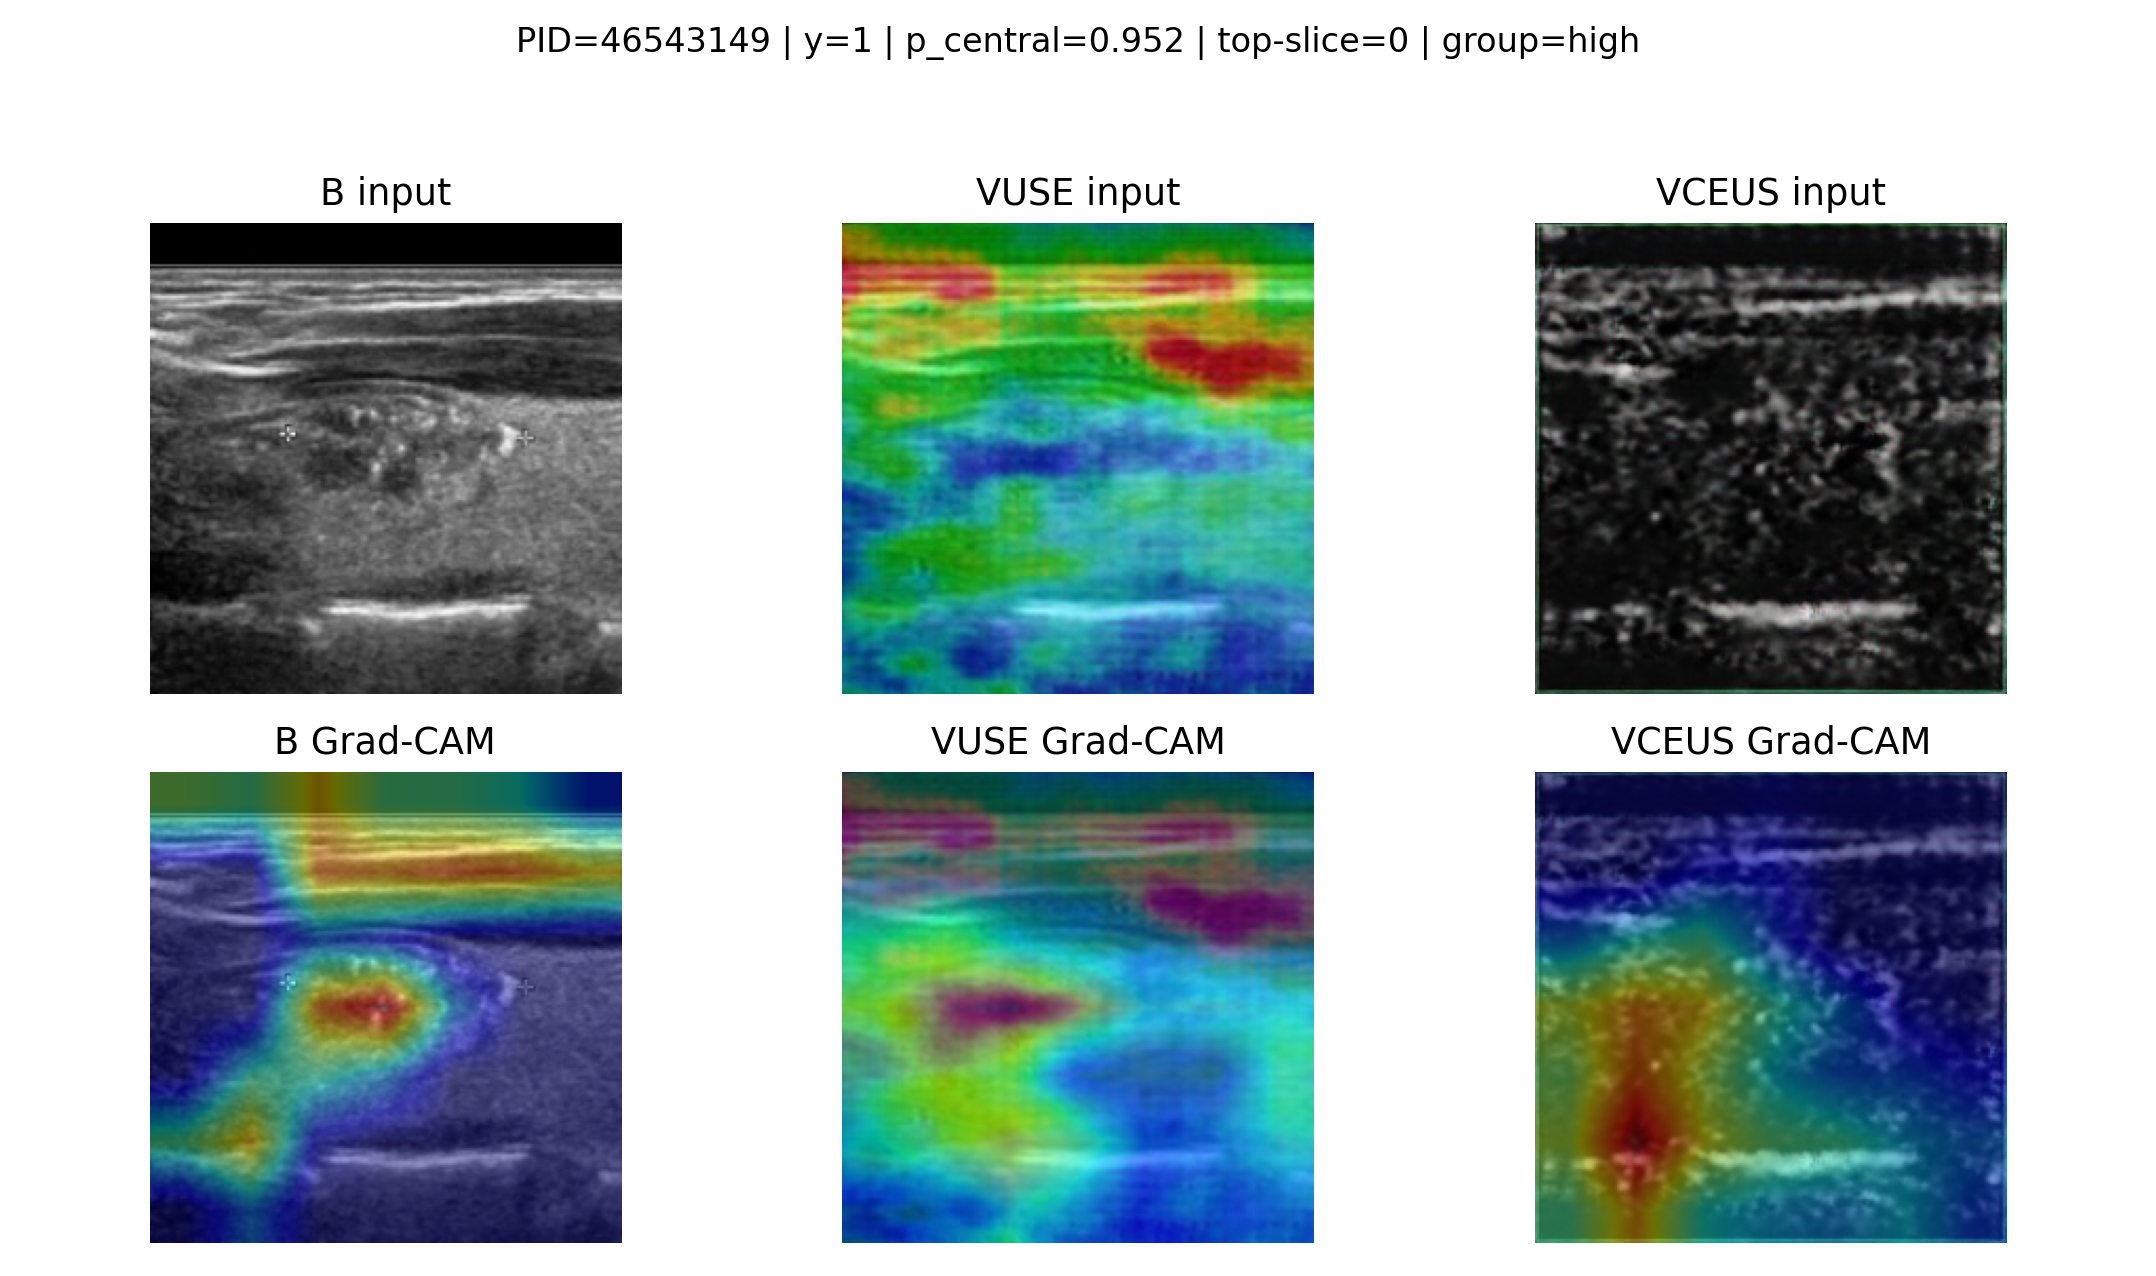
\includegraphics[width=0.92\textwidth]{figures/gradcam_modalities_case_high.png}
  \caption{高风险代表病例的多模态 Grad-CAM（同一高注意力切面）。}
\end{figure}
\paragraph{图表分析}在高风险病例中，不同模态对关键区域的响应强度与覆盖范围存在差异，提示多模态信息具备互补性。

\begin{figure}[H]
  \centering
  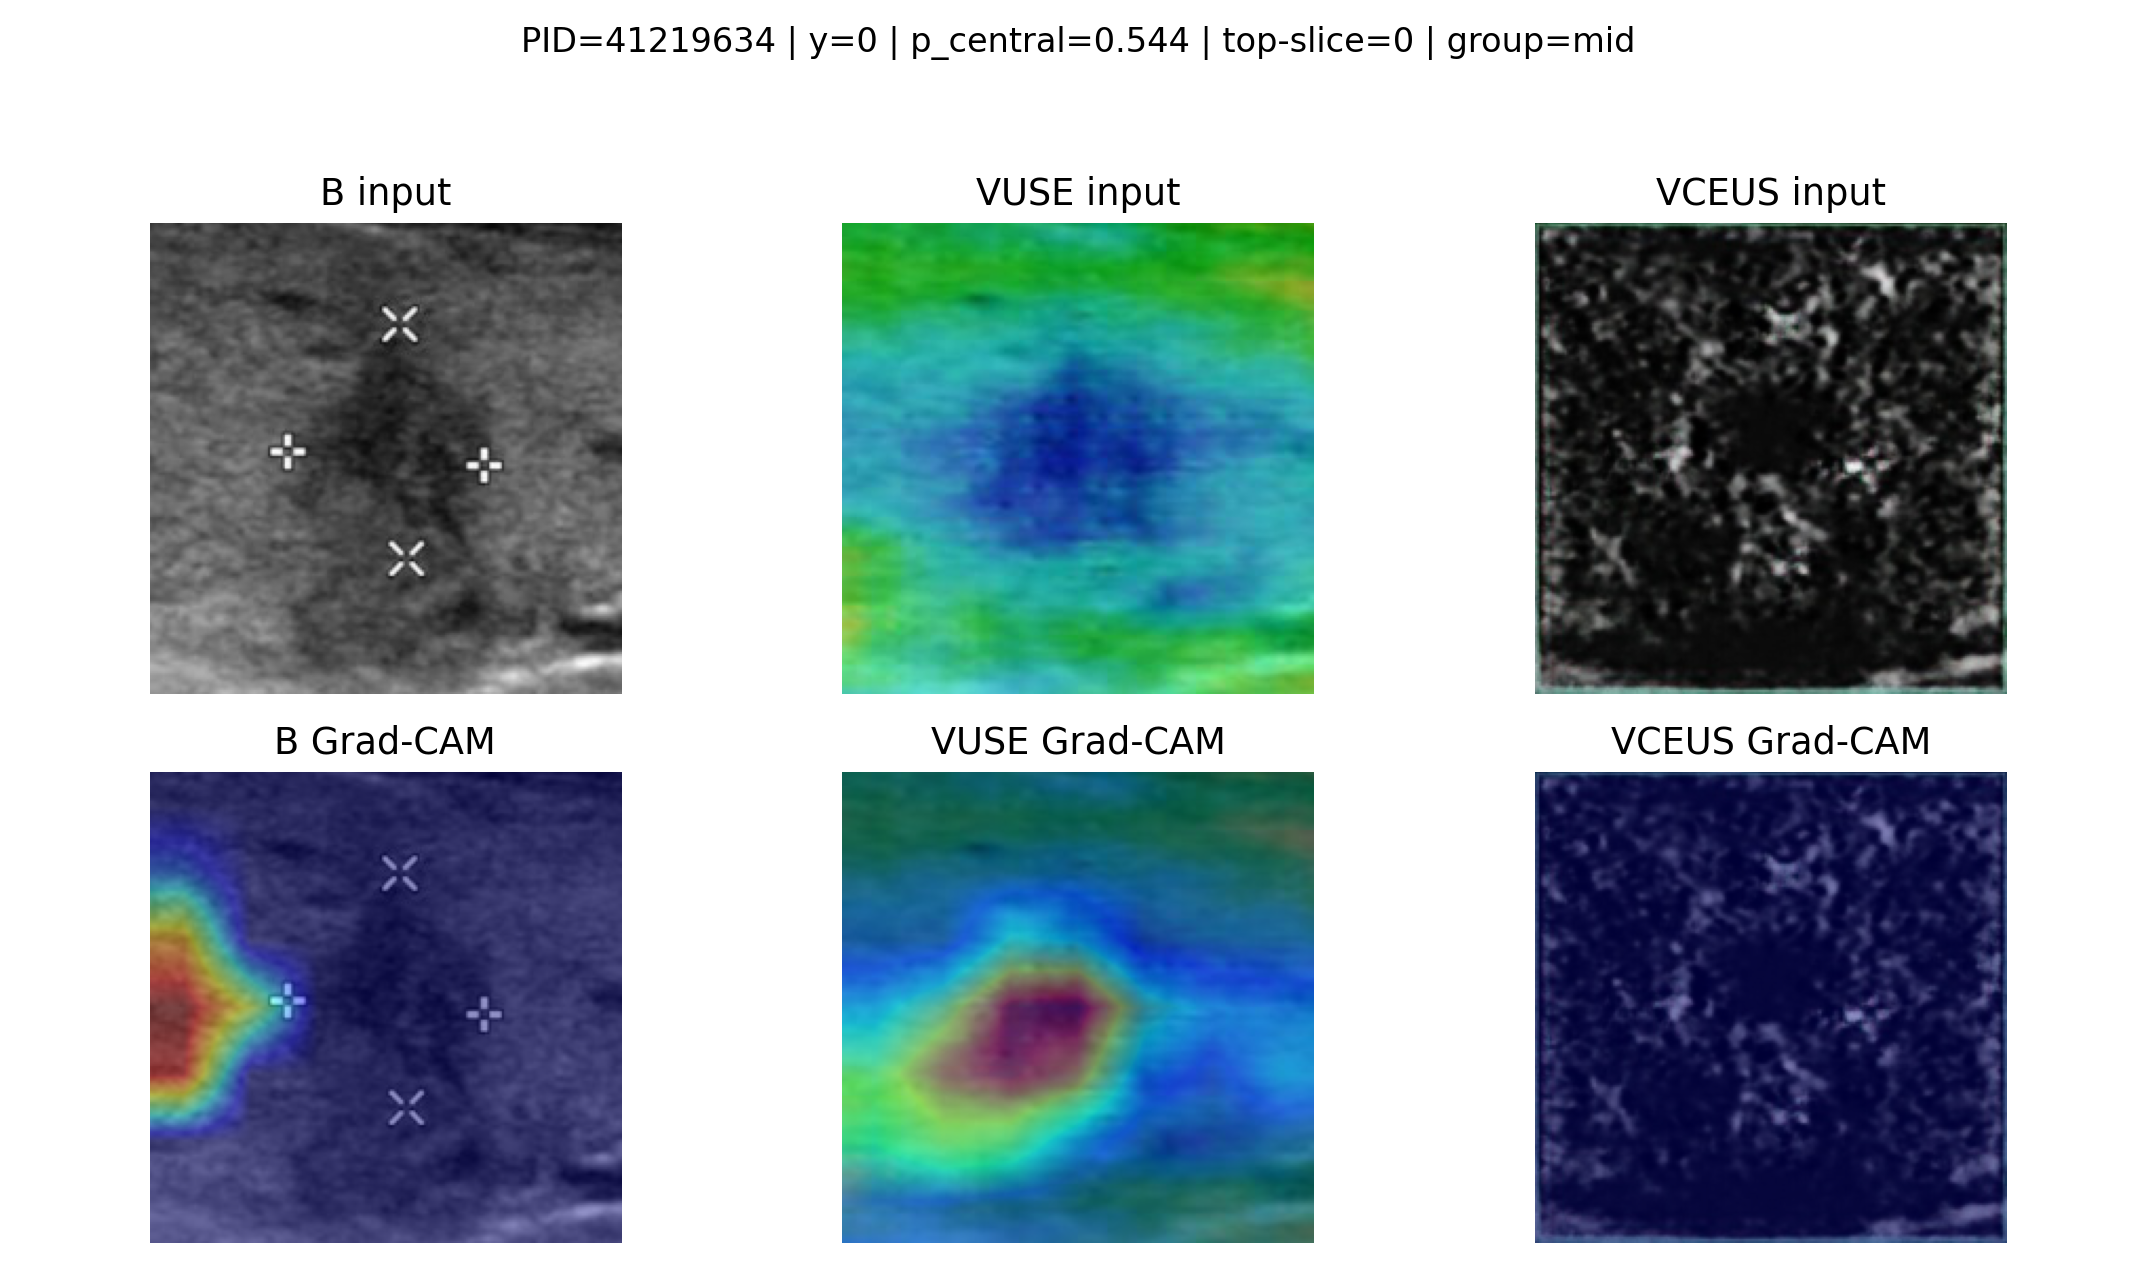
\includegraphics[width=0.92\textwidth]{figures/gradcam_modalities_case_mid.png}
  \caption{中风险代表病例的多模态 Grad-CAM。}
\end{figure}
\paragraph{图表分析}中风险病例的模态间分歧更明显，说明该类病例可能是融合策略最关键的增益区间。

\begin{figure}[H]
  \centering
  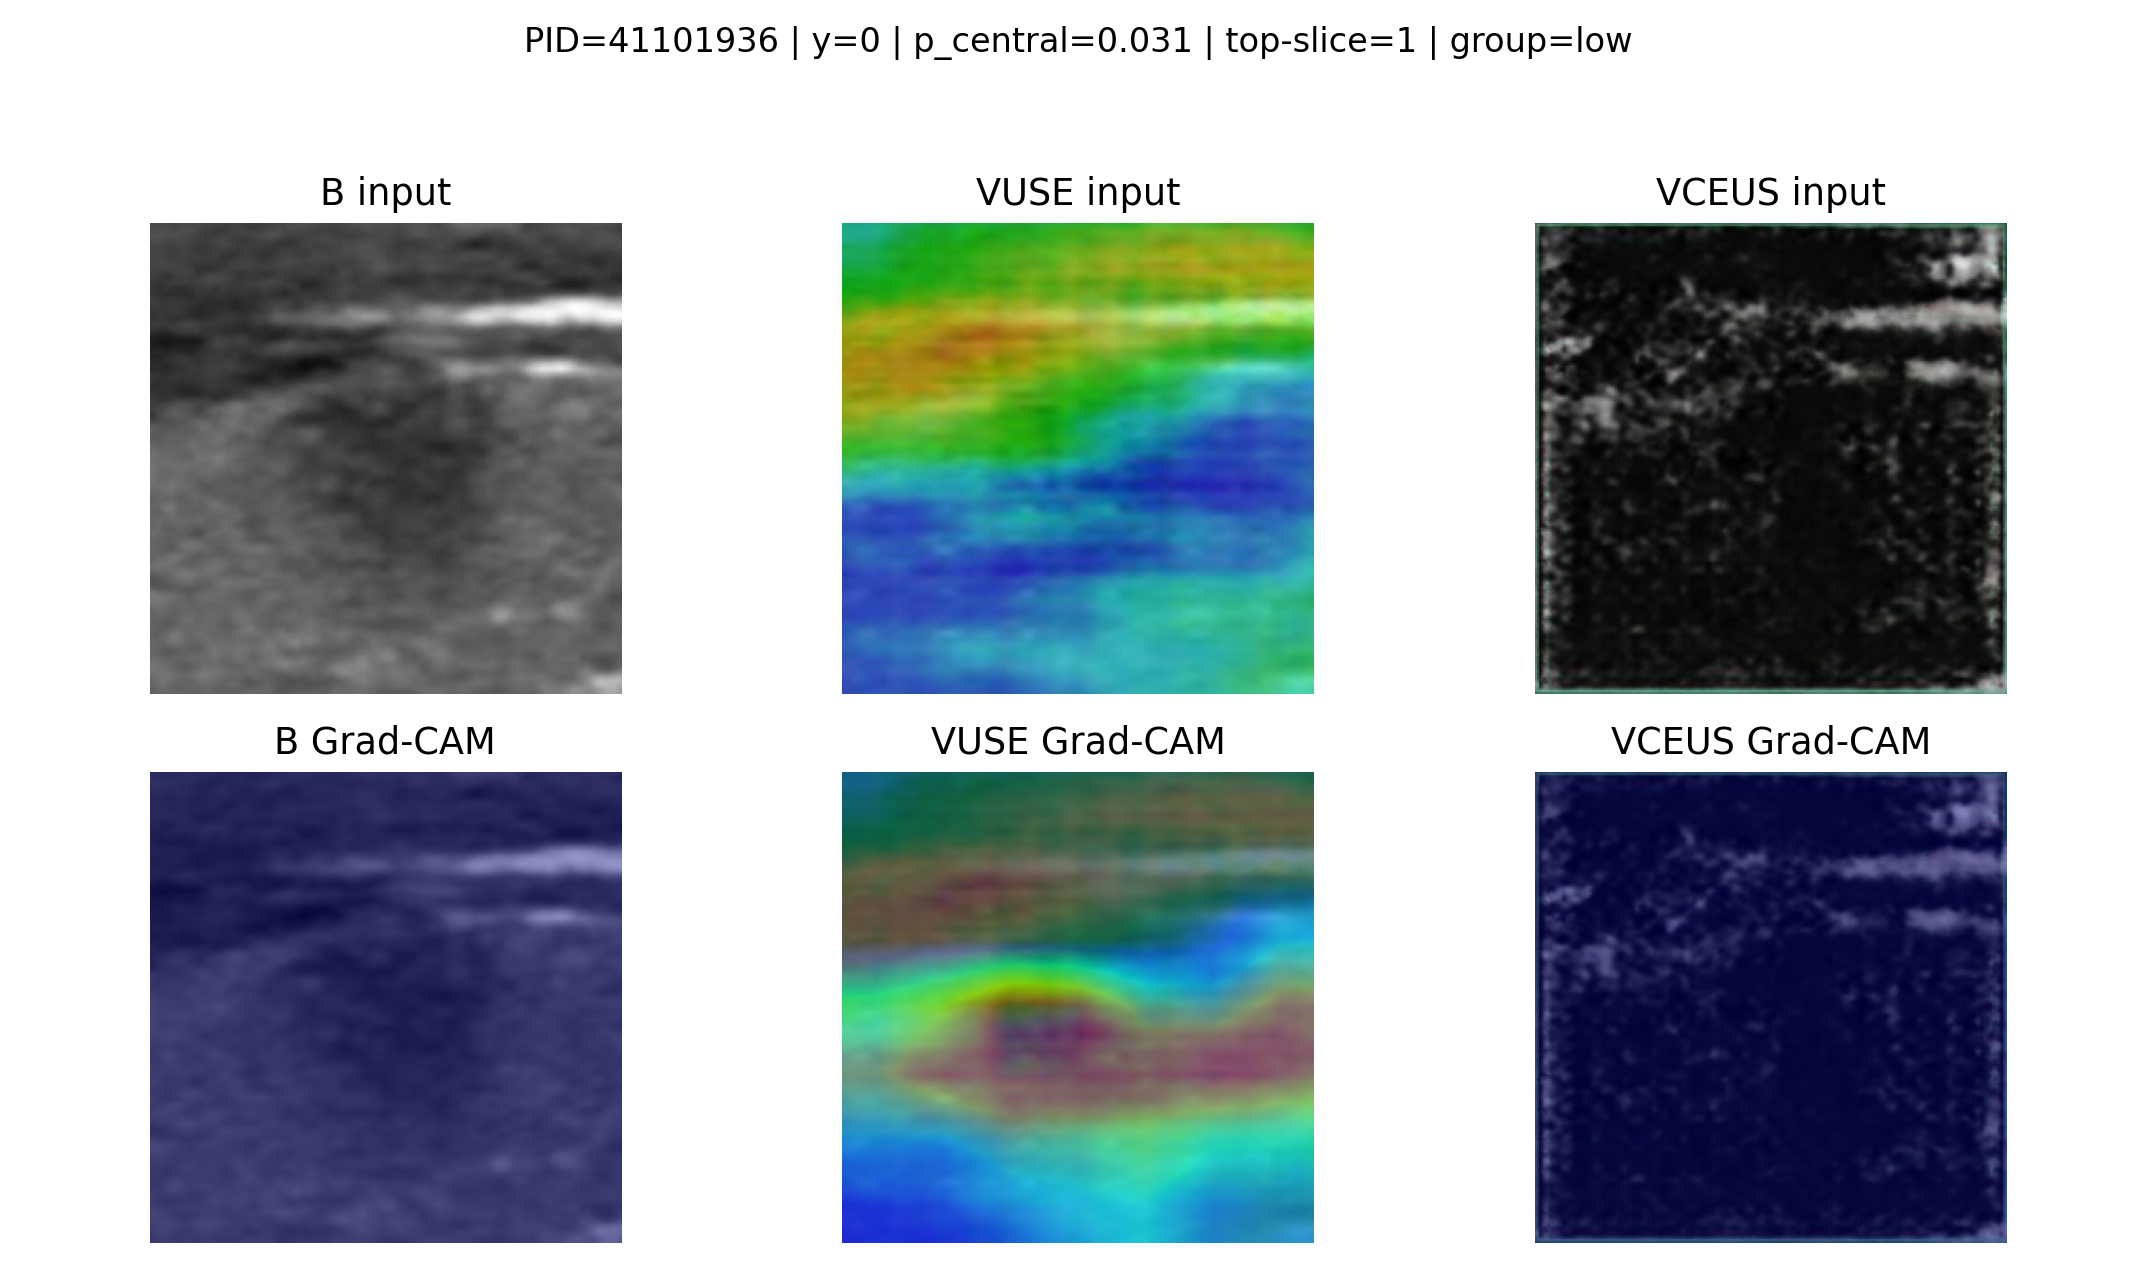
\includegraphics[width=0.92\textwidth]{figures/gradcam_modalities_case_low.png}
  \caption{低风险代表病例的多模态 Grad-CAM。}
\end{figure}
\paragraph{图表分析}低风险病例中多模态激活普遍较弱且缺乏一致高响应区域，符合低风险预测特征。

\paragraph{模态贡献对比观察}
从三类代表病例可见：B 模态更偏向结构边界响应，VUSE/VCEUS 在局部区域对比上提供补充证据。该现象支持“多模态并非简单冗余，而是病例依赖的互补贡献”。

\subsection{决策曲线分析（DCA）}
\begin{figure}[H]
  \centering
  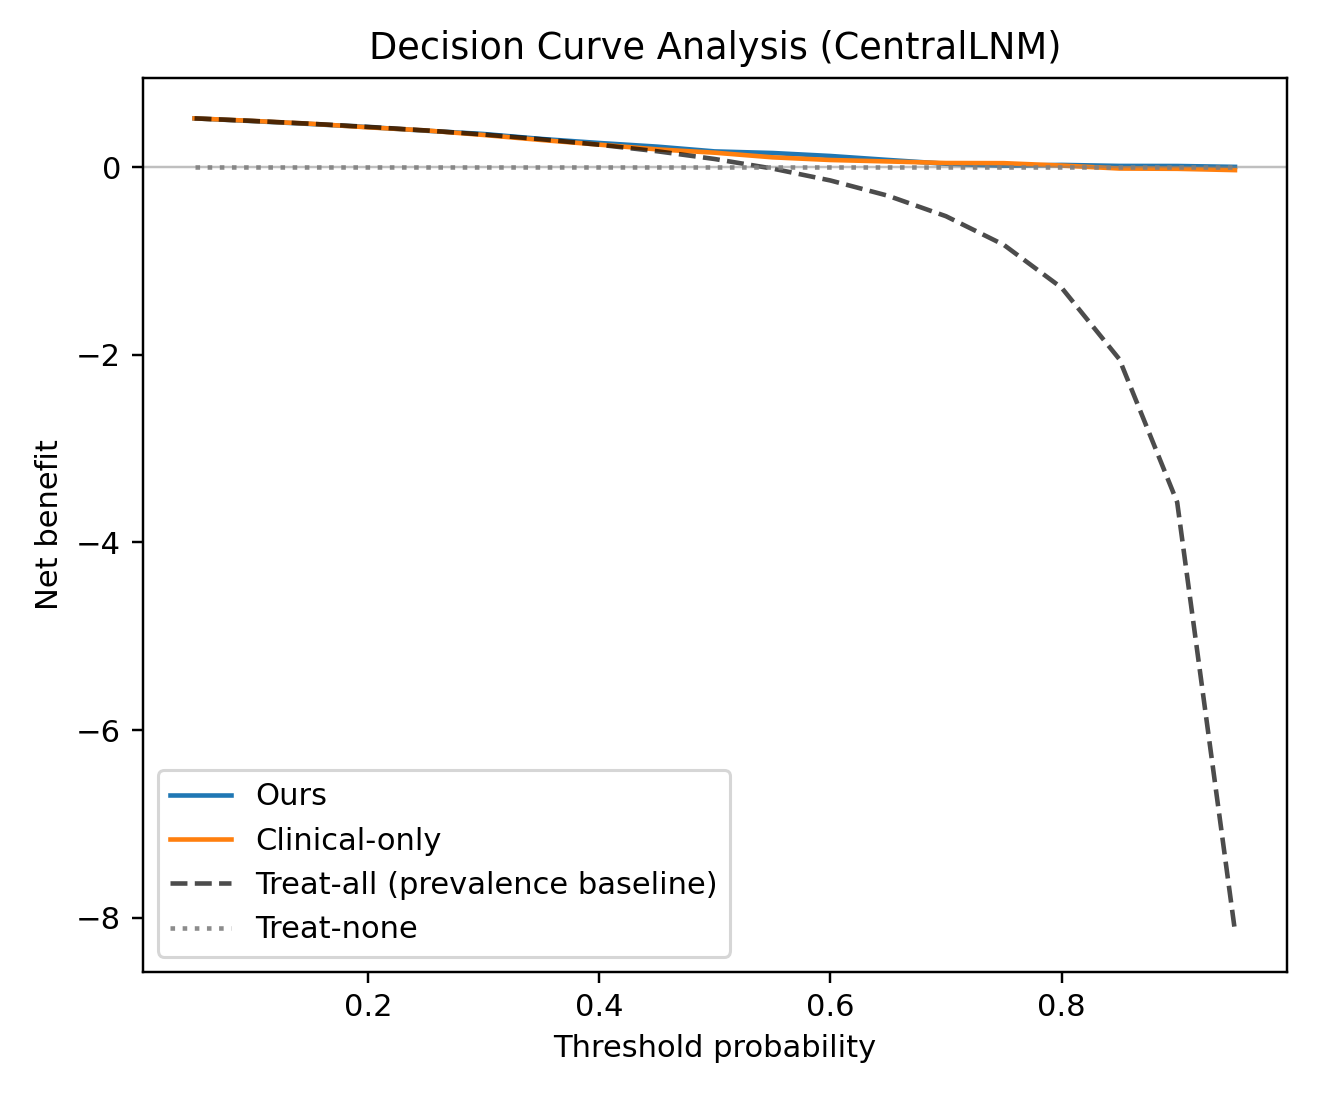
\includegraphics[width=0.68\textwidth]{figures/dca_ours_vs_clinical.png}
  \caption{Ours 与 Clinical-only 的 DCA 对比（叠加 treat-none 与 treat-all/prevalence 基线）。}
\end{figure}
\paragraph{图表分析}在主要阈值区间内，Ours 的净获益曲线整体高于 Clinical-only，体现更高临床决策收益。
\paragraph{图表分析}相较 treat-none 与 treat-all 基线，Ours 在中等阈值段表现更稳定，具有更优实用价值。

\subsection{校准分层表}
\begin{table}[H]
\centering
\small
\caption{Calibration strata of Ours (CentralLNM)}
\label{tab:calib_strata}
\begin{tabular}{p{0.24\textwidth}ccc}
\toprule
Risk bin ($\hat{p}_{central}$) & $N$ & Positive & Observed rate \\
\midrule
0.0$\sim$0.1 & 2 & 1 & 0.500 \\
0.1$\sim$0.2 & 9 & 2 & 0.222 \\
0.2$\sim$0.3 & 28 & 7 & 0.250 \\
0.3$\sim$0.4 & 38 & 16 & 0.421 \\
0.4$\sim$0.5 & 91 & 41 & 0.451 \\
0.5$\sim$0.6 & 122 & 62 & 0.508 \\
0.6$\sim$0.7 & 69 & 50 & 0.725 \\
0.7$\sim$0.8 & 47 & 33 & 0.702 \\
0.8$\sim$0.9 & 20 & 17 & 0.850 \\
0.9$\sim$1.0 & 5 & 5 & 1.000 \\
\bottomrule
\end{tabular}
\end{table}

\paragraph{表格分析}该表按预测概率区间统计真实阳性率（Observed rate），整体呈随风险分层升高而上升的趋势，说明模型输出概率具有可解释的分层能力。
\paragraph{表格分析}在高风险分层（如 0.8 以上）中阳性率显著更高，可支持术前“重点随访/强化评估”的临床决策；低风险分层则可辅助降低不必要干预。

\section{讨论}
（1）患者级建模相较切片级拼接的稳定性优势；（2）门控融合过滤影像噪声的作用及失效情境；（3）先验约束对临床一致性的贡献；（4）数据分布与域差异的潜在影响与后续缓解方案。

\section{局限与未来工作}
样本规模、类不平衡与域漂移；跨中心泛化与外部验证；注意力权重可解释性的更系统定量（留作后续补充图 —— “注意力权重分布与典型病例热力图”）。

\section{复现与开放}
代码与划分、训练日志与明细、图表与 Overleaf 文稿已在项目仓库中给出；新增脚本输出在 \texttt{HCP-Fusion Net/v2\_mil\_gated/} 与 \texttt{overleaf\_package\_mil/figures/}。

\appendix
\section{附录：Ablation 逐折明细表}
\begin{table}[H]
\centering
\small
\caption{Per-fold metrics: Baseline A (Clinical-only)}
\label{tab:baseline_a_clinical_only_per_fold}
\begin{tabular}{rrrrrr}
\toprule
fold & AUC & ACC & F1 & Sen & Spe \\
\midrule
0 & 0.640 & 0.563 & 0.513 & 0.426 & 0.725 \\
1 & 0.711 & 0.690 & 0.703 & 0.681 & 0.700 \\
2 & 0.632 & 0.547 & 0.589 & 0.596 & 0.487 \\
3 & 0.652 & 0.581 & 0.581 & 0.532 & 0.641 \\
4 & 0.702 & 0.671 & 0.745 & 0.891 & 0.410 \\
\bottomrule
\end{tabular}
\end{table}

\begin{table}[H]
\centering
\small
\caption{Per-fold metrics: Baseline B (Slice-Mean + Concat)}
\label{tab:baseline_b_slice_mean_concat_per_fold}
\begin{tabular}{rrrrrr}
\toprule
fold & AUC & ACC & F1 & Sen & Spe \\
\midrule
0 & 0.662 & 0.632 & 0.704 & 0.809 & 0.425 \\
1 & 0.657 & 0.540 & 0.630 & 0.723 & 0.325 \\
2 & 0.653 & 0.640 & 0.687 & 0.723 & 0.538 \\
3 & 0.661 & 0.570 & 0.602 & 0.596 & 0.538 \\
4 & 0.721 & 0.600 & 0.691 & 0.826 & 0.333 \\
\bottomrule
\end{tabular}
\end{table}

\begin{table}[H]
\centering
\small
\caption{Per-fold metrics: Ablation 1 (Mean-MIL + Gated)}
\label{tab:ablation1_mean_mil_gated_per_fold}
\begin{tabular}{rrrrrr}
\toprule
fold & AUC & ACC & F1 & Sen & Spe \\
\midrule
0 & 0.675 & 0.621 & 0.645 & 0.638 & 0.600 \\
1 & 0.708 & 0.644 & 0.680 & 0.702 & 0.575 \\
2 & 0.624 & 0.593 & 0.568 & 0.489 & 0.718 \\
3 & 0.669 & 0.616 & 0.560 & 0.447 & 0.821 \\
4 & 0.713 & 0.659 & 0.707 & 0.761 & 0.538 \\
\bottomrule
\end{tabular}
\end{table}

\begin{table}[H]
\centering
\small
\caption{Per-fold metrics: Ablation 2 (Attention-MIL + Concat)}
\label{tab:ablation2_attention_mil_concat_per_fold}
\begin{tabular}{rrrrrr}
\toprule
fold & AUC & ACC & F1 & Sen & Spe \\
\midrule
0 & 0.637 & 0.609 & 0.679 & 0.766 & 0.425 \\
1 & 0.705 & 0.655 & 0.659 & 0.617 & 0.700 \\
2 & 0.654 & 0.593 & 0.653 & 0.702 & 0.462 \\
3 & 0.641 & 0.605 & 0.605 & 0.553 & 0.667 \\
4 & 0.700 & 0.612 & 0.686 & 0.783 & 0.410 \\
\bottomrule
\end{tabular}
\end{table}

\begin{table}[H]
\centering
\small
\caption{Per-fold metrics: Ablation 3 (No Prior Constraint)}
\label{tab:ablation3_no_penalty_per_fold}
\begin{tabular}{rrrrrr}
\toprule
fold & AUC & ACC & F1 & Sen & Spe \\
\midrule
0 & 0.693 & 0.598 & 0.588 & 0.532 & 0.675 \\
1 & 0.690 & 0.552 & 0.678 & 0.872 & 0.175 \\
2 & 0.625 & 0.581 & 0.600 & 0.574 & 0.590 \\
3 & 0.665 & 0.593 & 0.607 & 0.574 & 0.615 \\
4 & 0.686 & 0.612 & 0.718 & 0.913 & 0.256 \\
\bottomrule
\end{tabular}
\end{table}

\begin{table}[H]
\centering
\small
\caption{Per-fold metrics: Ours (Attention-MIL + Gated + Prior)}
\label{tab:ours_full_per_fold}
\begin{tabular}{rrrrrr}
\toprule
fold & AUC & ACC & F1 & Sen & Spe \\
\midrule
0 & 0.680 & 0.598 & 0.632 & 0.638 & 0.550 \\
1 & 0.691 & 0.563 & 0.667 & 0.809 & 0.275 \\
2 & 0.699 & 0.663 & 0.695 & 0.702 & 0.615 \\
3 & 0.715 & 0.663 & 0.713 & 0.766 & 0.538 \\
4 & 0.696 & 0.635 & 0.667 & 0.674 & 0.590 \\
\bottomrule
\end{tabular}
\end{table}


\end{document}
